\documentclass[
    11pt,
    oneside, %  comment to switch to alternatig margins (for printed layout)
    english,
    singlespacing, % Single line spacing, alternatives: onehalfspacing or doublespacing
%draft, % Uncomment to enable draft mode (no pictures, no links, overfull hboxes indicated)
%nolistspacing, % If the document is onehalfspacing or doublespacing, uncomment this to set spacing in lists to single
%liststotoc, % Uncomment to add the list of figures/tables/etc to the table of contents
%toctotoc, % Uncomment to add the main table of contents to the table of contents
parskip, % Uncomment to add space between paragraphs
%nohyperref, % Uncomment to not load the hyperref package
    headsepline, % Uncomment to get a line under the header
%chapterinoneline, % Uncomment to place the chapter title next to the number on one line
%consistentlayout, % Uncomment to change the layout of the declaration, abstract and acknowledgements pages to match the default layout
]{MastersDoctoralThesis}

\usepackage[utf8]{inputenc}
\usepackage[T1]{fontenc}
\usepackage[nodayofweek]{datetime}
\usepackage{mathpazo}
%\usepackage{fontspec}
%\setmonofont{Consolas}

%\usepackage{pgfgantt}
\usepackage[backend=bibtex,style=vancouver,natbib=true]{biblatex} % Use the bibtex backend with the authoryear citation style (which resembles APA)

\addbibresource{biblio.bib}

\usepackage[autostyle=true]{csquotes}
\usepackage{tikz}
\usetikzlibrary{shapes.misc, arrows.meta}
\usepackage{amsmath}
\usepackage{amsthm}
\usepackage{textcomp}
\usepackage{color}
\usepackage{markdown}
\usepackage{wasysym}
\usepackage{amssymb}
\usetikzlibrary{arrows,positioning}
%\tikzset{
%%Define standard arrow tip
%    >=stealth',
%%Define style for boxes
%    punkt/.style={
%        rectangle,
%        rounded corners,
%        draw=black, thick,
%        text width=6.5em,
%        minimum height=2em,
%        text centered},
%% Define arrow style
%    pil/.style={
%        ->,
%        thick,
%        shorten <=2pt,
%        shorten >=2pt,}
%}
\geometry{
    paper=a4paper,
    inner=2.8cm,
    outer=2.8cm,
    bindingoffset=.5cm,
    top=1.5cm,
    bottom=1.5cm,
%showframe, % Uncomment to show how the type block is set on the page
}

% personal macros

\newcommand{\citeTODO}{[\scriptsize{\textit{\textsc{CITATION NEEDED}}}\normalsize]}
\newdateformat{daymonth}{
    \ordinal{DAY}\ of \monthname[\THEMONTH]
}
\newcommand{\monthdate}[2]{ \daymonth\formatdate{#1}{#2}{2022}}
% TODO find a nice definition format
\theoremstyle{definition}
\newtheorem{definition}{Definition}
\providecommand*\definitionautorefname{Definition}
\providecommand*{\listingautorefname}{Listing}


%
%\newcommand{\thickerhline}{
%    \setlength{\arrayrulewidth}{.11.6.105em}
%    \hline
%    \setlength{\arrayrulewidth}{.05em}
%}

%\thesistitle{Exploring Trustless Licensing} % print with \ttitle
\thesistitle {Confis: A Framework for Authoring and Querying Machine-Readable Legal Agreements}
\supervisor{Prof. William J. \textsc{Knottenbelt}} % print with \supname
\marker{Dr. Paul A. \textsc{Bilokon}}
\degree{MEng Computing} % print with \degreename
\author{Nicolás \textsc{D'Cotta}} % print with \authorname
\addresses{} % print with \addressname

\subject{Computer Science} % Your subject area, this is not currently used anywhere in the template, print it elsewhere with \subjectname
\keywords{} % TODO fill - print with \keywordnames
\university{\href{https://www.imperial.ac.uk/}{Imperial College London}} % Your university's name and URL, this is used in the title page and abstract, print it elsewhere with \univname
\department{\href{https://www.imperial.ac.uk/computing}{Department of Computing}} % Your department's name and URL, this is used in the title page and abstract, print it elsewhere with \deptname
\group{\href{https://researchgroup.university.com}{Research Group Name}} % Your research group's name and URL, this is used in the title page, print it elsewhere with \groupname
\faculty{\href{https://faculty.university.com}{Faculty of Engineering}} % Your faculty's name and URL, this is used in the title page and abstract, print it elsewhere with \facname

\AtBeginDocument{
    \hypersetup{pdftitle=\ttitle} % Set the PDF's title to your title
    \hypersetup{pdfauthor=\authorname} % Set the PDF's author to your name
    \hypersetup{pdfkeywords=\keywordnames} % Set the PDF's keywords to your keywords
}


\begin{document}
    \usemintedstyle{tango}
    \frontmatter
    \pagestyle{plain}

%----------------------------------------------------------------------------------------
%	TITLE PAGE
%----------------------------------------------------------------------------------------

    \begin{titlepage}
        \begin{center}

            \vspace*{.06\textheight}
            {\scshape\LARGE \univname\par}\vspace{1.5cm}
            % TODO restore for report
            \textsc{\Large MEng Final Year Project}\\[0.5cm]

            \HRule \\[0.4cm]
            {\huge \bfseries \ttitle\par}\vspace{0.4cm} % Thesis title
            \HRule \\[1.5cm]

            \begin{minipage}[t]{0.4\textwidth}
                \begin{flushleft}
                    \large
                    \emph{Author:}\\
                    \href{https://nico.dcotta.eu}{\authorname}
                \end{flushleft}
            \end{minipage}
            \begin{minipage}[t]{0.4\textwidth}
                \begin{flushright}
                    \large
                    \emph{Supervisor:} \\
                    \href{https://www.doc.ic.ac.uk/~wjk/}{\supname} \\[0.4 cm]
                    \emph{Second Marker:} \\
                    \href{https://www.imperial.ac.uk/people/paul.bilokon01}{\markername}
                \end{flushright}
            \end{minipage}\\[3cm]

            \vfill
            \large \textit{A report submitted in fulfillment of the requirements\\ for the degree of \degreename}\\[0.3cm] % University requirement text
            \textit{in the}\\[0.4 cm]
            \facname \\ \deptname\\[2 cm]

            \vfill

            {\large \today}\\[4cm] % Date
%\includegraphics{Logo} % University/department logo - uncomment to place it

            \vfill
        \end{center}
    \end{titlepage}


    \begin{abstract}
        \addchaptertocentry{\abstractname} % Add the abstract to the table of contents

        % make it clear why you I am trying to operationalise contracts
        % - make it easier to exploit digital form of the contract
        % - give people an understanding of capabilities, exposures, obligations wrt contracts

        % no technologies succeed at helping us understand a contract
        % lots of automation tech around contracts but it focuses on bureaucratic overheads (such as signing, version control, and proof of existence).


        For more than four thousand years, humankind has utilised contracts to govern economic activity.
        Since their conception in ancient times, they have been represented as clauses of natural language and how we reason about them has remained unchanged, despite technological leaps and civilization's dependence on them.
        In the last few decades, since the seminal work on smart contracts by Szabo in 1997, the benefits of formalising and automating contracts have become increasingly obvious.
        Such benefits include making it easier for parties to understand the legal constraints they are under, as well as the capabilities they have.

        % missing direction of travel at the end of 1st paragrapgh

        % there are lots of contracts -> they are nat language -> how we reason about them has remained unchanged since their conception 3 thousand years ago


        Rather than replacing existing legal infrastructure, some new technologies like blockchain-based smart contracts have created a new class of self-enforcing software systems which mostly revolve around financial products.
        Other, more logic-based attempts to automate reasoning with legal documents are very specialist and require understanding of advanced topics, such as logic programming, linear temporal logic, or the event calculus;
        and are not self-contained solutions.
        This lack of accessibility of existing technologies means that they have not seen practical adoption in industry.

        This project introduces \textbf{\emph{Confis}}, a Kotlin-based accessible language that specifies legal agreements and immediately answers complex queries.
%        Its features include converting documents back to plain English, an intelligent editor with a live preview, and a user interface for performing complex queries on documents as they are written.
        Contracts are written as stand-alone scripts inside a fully-capable editor based on IntelliJ IDEA, inside which a live preview displays a plain English render of the encoded agreement.
        In stark contrast with the state of the art, Confis does not require engineering, logical, nor legal expertise for its effective use.
        A graphical UI allows making questions involving parties' legal capabilities and their compliance, such as \emph{`What needs to happen for my landlord evict me?'} or \emph{`Has the seller breached our agreement?'} -- which Confis is able to answer in plain English.


        % something in this technical paragraph about architecture ^
        % showcase your technical achievement!

%        The result is an end-to-end framework that provides abstractions that successfully represents a broad range of contracts, comparable to Symboleo or The Accord Project, except with a strong focus on accessibility and ease-of-use aimed at industry.
%        Simple and easier to learn abstractions are brought forward by compromising mainly on language expressiveness -- and therefore in the complexity of the contracts that can be represented.

        % Last paragraph is kind of queries
        Overall, this project operationalises legal agreements by providing the industry with relevant and pragmatic tools.
        By formalising the fewest key abstractions, we prove it successfully represents common classes of contracts (such as licenses and sales agreements) much like Symboleo or The Accord project -- except with a strong focus on accessibility and through a self-contained solution.
        Confis also succeeds at avoiding exposing advanced complexities that hinder its accessibility, by compromising on language expressiveness.
        We show this accessibility is at the price of not being able to formalise some more specific legal scenarios, which limits the range of contracts Confis can specify.

        Next steps include communicating with other services for them to be aware of their legal capabilities (rather than relying on legal advice across teams inside an organisation), as well as improving the compromise between the contracts that can be represented and the complexity of the language.
        % specify how you built on top of another lang as an internal DSL

        % last para did you manage succesfully?? what about the future of contracts in general
        % what works what does not work
        % general outlook

        % what case studies

    \end{abstract}


    \begin{acknowledgements}
        \addchaptertocentry{\acknowledgementname} % TODO write akcnowledgements
        I would like to thank William, my supervisor\dots.
    \end{acknowledgements}

    \tableofcontents
    \listoffigures
    \listoftables
    \listoflistings

%    \setlength{\parskip}{\medskipamount}
    \setlength{\parindent}{0pt}


    \mainmatter % Begin numeric (1,2,3...) page numbering

    \pagestyle{thesis} % Return the page headers back to the "thesis" style


    \chapter{Introduction}\label{ch:introduction}

\section{Main Section 1}

Lorem ipsum dolor sit amet, consectetur adipiscing elit. Aliquam ultricies lacinia euismod. Nam tempus risus in dolor rhoncus in interdum enim tincidunt. Donec vel nunc neque. In condimentum ullamcorper quam non consequat. Fusce sagittis tempor feugiat. Fusce magna erat, molestie eu convallis ut, tempus sed arcu. Quisque molestie, ante a tincidunt ullamcorper, sapien enim dignissim lacus, in semper nibh erat lobortis purus. Integer dapibus ligula ac risus convallis pellentesque.

\subsection{Subsection 1}

Nunc posuere quam at lectus tristique eu ultrices augue venenatis. Vestibulum ante ipsum primis in faucibus orci luctus et ultrices posuere cubilia Curae; Aliquam erat volutpat. Vivamus sodales tortor eget quam adipiscing in vulputate ante ullamcorper. Sed eros ante, lacinia et sollicitudin et, aliquam sit amet augue. In hac habitasse platea dictumst.


\subsection{Subsection 2}
Morbi rutrum odio eget arcu adipiscing sodales. Aenean et purus a est pulvinar pellentesque. Cras in elit neque, quis varius elit. Phasellus fringilla, nibh eu tempus venenatis, dolor elit posuere quam, quis adipiscing urna leo nec orci. Sed nec nulla auctor odio aliquet consequat. Ut nec nulla in ante ullamcorper aliquam at sed dolor. Phasellus fermentum magna in augue gravida cursus. Cras sed pretium lorem. Pellentesque eget ornare odio. Proin accumsan, massa viverra cursus pharetra, ipsum nisi lobortis velit, a malesuada dolor lorem eu neque.

\section{Main Section 2}

Sed ullamcorper quam eu nisl interdum at interdum enim egestas. Aliquam placerat justo sed lectus lobortis ut porta nisl porttitor. Vestibulum mi dolor, lacinia molestie gravida at, tempus vitae ligula. Donec eget quam sapien, in viverra eros. Donec pellentesque justo a massa fringilla non vestibulum metus vestibulum. Vestibulum in orci quis felis tempor lacinia. Vivamus ornare ultrices facilisis. Ut hendrerit volutpat vulputate. Morbi condimentum venenatis augue, id porta ipsum vulputate in. Curabitur luctus tempus justo. Vestibulum risus lectus, adipiscing nec condimentum quis, condimentum nec nisl. Aliquam dictum sagittis velit sed iaculis. Morbi tristique augue sit amet nulla pulvinar id facilisis ligula mollis. Nam elit libero, tincidunt ut aliquam at, molestie in quam. Aenean rhoncus vehicula hendrerit.


\section{Main Section 3}

Thanks for assisting to my TED talk.

    \chapter{Background}\label{ch:background}


\section{Cryptography Primitives}\label{sec:cryptography}

\subsection{Hash Functions}\label{subsec:crypto:hash}

Hash functions are cryptographic functions designed to behave like random
functions~\cite{smart2016randomOracleModel}.
When building a security proof, they can be assumed to have the following properties~\cite{smart2016randomOracleModel,
    smart2016hashFunctions}:
% FIXME needs references
\begin{description}
    \item[Determinism] A hash function always produces the same output for the same input
    \item[One-way] It is computationally impossible to compute the preimage for some output of a hash function
    \item[Uniformity] Outputs of a hash function are expected to be uniformly distributed.
    In practice, the output space of a hash function is finite, so \textit{collisions} (where two inputs produce the
    same output) are possible, but uniformity ensures this is an unlikely scenario.
\end{description}

\subsection{Symmetric key cryptography}

% TODO will i need this

\subsection{Public Key Cryptography}\label{subsec:crypto:pubkey}

In public key cryptography, two communicating parties (say Alice and Bob) can communicate privately by using pairs of
numbers that are related mathematically and which allow converting cleartext into cyphertext and
back~\cite{smart2016publicKey}.
This pair of numbers is called an asymmetric keypair, and is composed of a \textbf{public key} $e$ and a \textbf{private
key} $d$.\\

In this example, if Alice wishes to communicate with Bob, Bob can generate a keypair $(d, e)$ and publish $e$.
Alice can then encrypt her cleartext with $e$, and only Bob will be able to decrypt it (because only Bob knows $d$).

\begin{figure}[th]
    \centering
    \tikzset{every picture/.style={line width=0.75pt}} %set default line width to 0.75pt
    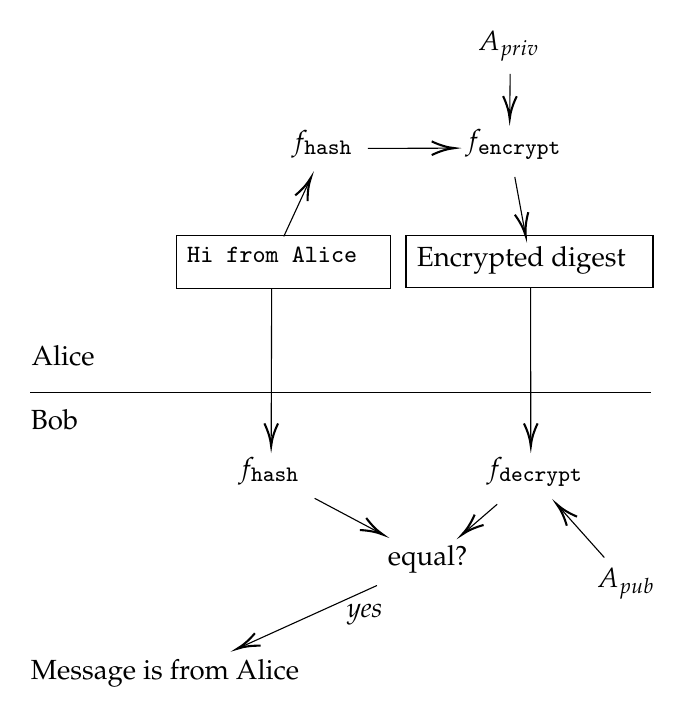
\begin{tikzpicture}[x=0.75pt,y=0.75pt,yscale=-1,xscale=1]
%uncomment if require: \path (0,355); %set diagram left start at 0, and has height of 355

%Straight Lines [id:da017592532205451983]
        \draw    (60.54,179.69) -- (359.87,179.69) ;

% Text Node
        \draw    (131,104) -- (234,104) -- (234,129.67) -- (131,129.67) -- cycle ;
        \draw (135,108.67) node [anchor=north west][inner sep=0.75pt]   [align=left] {\small \texttt{Hi from Alice}};
% Text Node
        \draw (185.33,52.33) node [anchor=north west][inner sep=0.75pt]   [align=left] {$\displaystyle f_{\texttt{hash}}$};
% Text Node
        \draw (275,4.33) node [anchor=north west][inner sep=0.75pt]   [align=left] {$\displaystyle A_{priv}$};
% Text Node
        \draw (332.33,263.33) node [anchor=north west][inner sep=0.75pt]   [align=left] {$\displaystyle A_{pub}$};
% Text Node
        \draw (269,52) node [anchor=north west][inner sep=0.75pt]   [align=left] {$\displaystyle f_{\texttt{encrypt}}$};
% Text Node
        \draw    (241.67,104) -- (360.67,104) -- (360.67,129.33) -- (241.67,129.33) -- cycle ;
        \draw (245.67,108.33) node [anchor=north west][inner sep=0.75pt]   [align=left] {Encrypted digest};
% Text Node
        \draw (60,156) node [anchor=north west][inner sep=0.75pt]   [align=left] {Alice};
% Text Node
        \draw (59.67,186.67) node [anchor=north west][inner sep=0.75pt]   [align=left] {Bob};
% Text Node
        \draw (159.67,209.67) node [anchor=north west][inner sep=0.75pt]   [align=left] {$\displaystyle f_{\texttt{hash}}$};
% Text Node
        \draw (279.33,209.67) node [anchor=north west][inner sep=0.75pt]   [align=left] {$\displaystyle f_{\texttt{decrypt}}$};
% Text Node
        \draw (231.67,252.33) node [anchor=north west][inner sep=0.75pt]   [align=left] {equal?};
% Text Node
        \draw (59.67,307.33) node [anchor=north west][inner sep=0.75pt]   [align=left] {Message is from Alice};
% Text Node
        \draw (208.67,280.33) node [anchor=north west][inner sep=0.75pt]   [align=left] {\textit{{ yes}}};
% Connection
        \draw    (182.78,104.67) -- (195.03,78.15) ;
        \draw [shift={(195.87,76.33)}, rotate = 114.8] [color={rgb, 255:red, 0; green, 0; blue, 0 }  ][line width=0.75]    (10.93,-3.29) .. controls (6.95,-1.4) and (3.31,-0.3) .. (0,0) .. controls (3.31,0.3) and (6.95,1.4) .. (10.93,3.29)   ;
% Connection
        \draw    (223.33,62.25) -- (263,62.11) ;
        \draw [shift={(265,62.1)}, rotate = 179.79] [color={rgb, 255:red, 0; green, 0; blue, 0 }  ][line width=0.75]    (10.93,-3.29) .. controls (6.95,-1.4) and (3.31,-0.3) .. (0,0) .. controls (3.31,0.3) and (6.95,1.4) .. (10.93,3.29)   ;
% Connection
        \draw    (294.1,76) -- (298.98,102.37) ;
        \draw [shift={(299.35,104.33)}, rotate = 259.5] [color={rgb, 255:red, 0; green, 0; blue, 0 }  ][line width=0.75]    (10.93,-3.29) .. controls (6.95,-1.4) and (3.31,-0.3) .. (0,0) .. controls (3.31,0.3) and (6.95,1.4) .. (10.93,3.29)   ;
% Connection
        \draw    (291.87,26.33) -- (291.66,46) ;
        \draw [shift={(291.64,48)}, rotate = 270.59] [color={rgb, 255:red, 0; green, 0; blue, 0 }  ][line width=0.75]    (10.93,-3.29) .. controls (6.95,-1.4) and (3.31,-0.3) .. (0,0) .. controls (3.31,0.3) and (6.95,1.4) .. (10.93,3.29)   ;
% Connection
        \draw    (176.96,129.67) -- (176.72,203.67) ;
        \draw [shift={(176.71,205.67)}, rotate = 270.19] [color={rgb, 255:red, 0; green, 0; blue, 0 }  ][line width=0.75]    (10.93,-3.29) .. controls (6.95,-1.4) and (3.31,-0.3) .. (0,0) .. controls (3.31,0.3) and (6.95,1.4) .. (10.93,3.29)   ;
% Connection
        \draw    (301.69,129.33) -- (301.81,203.67) ;
        \draw [shift={(301.81,205.67)}, rotate = 269.91] [color={rgb, 255:red, 0; green, 0; blue, 0 }  ][line width=0.75]    (10.93,-3.29) .. controls (6.95,-1.4) and (3.31,-0.3) .. (0,0) .. controls (3.31,0.3) and (6.95,1.4) .. (10.93,3.29)   ;
% Connection
        \draw    (197.67,230.82) -- (228.87,247.4) ;
        \draw [shift={(230.63,248.33)}, rotate = 207.98] [color={rgb, 255:red, 0; green, 0; blue, 0 }  ][line width=0.75]    (10.93,-3.29) .. controls (6.95,-1.4) and (3.31,-0.3) .. (0,0) .. controls (3.31,0.3) and (6.95,1.4) .. (10.93,3.29)   ;
% Connection
        \draw    (285.62,233.67) -- (270.15,247.03) ;
        \draw [shift={(268.64,248.33)}, rotate = 319.18] [color={rgb, 255:red, 0; green, 0; blue, 0 }  ][line width=0.75]    (10.93,-3.29) .. controls (6.95,-1.4) and (3.31,-0.3) .. (0,0) .. controls (3.31,0.3) and (6.95,1.4) .. (10.93,3.29)   ;
% Connection
        \draw    (227.67,272.83) -- (162.1,302.51) ;
        \draw [shift={(160.28,303.33)}, rotate = 335.64] [color={rgb, 255:red, 0; green, 0; blue, 0 }  ][line width=0.75]    (10.93,-3.29) .. controls (6.95,-1.4) and (3.31,-0.3) .. (0,0) .. controls (3.31,0.3) and (6.95,1.4) .. (10.93,3.29)   ;
% Connection
        \draw    (337.23,259.33) -- (315.66,235.16) ;
        \draw [shift={(314.33,233.67)}, rotate = 48.25] [color={rgb, 255:red, 0; green, 0; blue, 0 }  ][line width=0.75]    (10.93,-3.29) .. controls (6.95,-1.4) and (3.31,-0.3) .. (0,0) .. controls (3.31,0.3) and (6.95,1.4) .. (10.93,3.29)   ;

    \end{tikzpicture}
    \decoRule
    \caption[Asymmetric signing scheme]{An asymmetric key signing scheme where Bob is able to verify only Alice could
    have written '\texttt{Hi from Alice}'}
    \label{fig:pubkey-signing}
\end{figure}

Conversely, the same keypair can be used by Bob to send a message to Alice where Alice can verify that only Bob
could have written the message.
This is called \textit{signing}~\cite{smart2016signatures} and, more generally, it allows a sender of a message to
prove they are the authors of the message to a recipient.
An example of a signing scheme can be seen in Figure~\ref{fig:pubkey-signing}.

\subsection{Secure Digital Timestamps}\label{subsec:crypto:timestamps}
% TODO citation for definiton
\textit{Trusted (digital) timestamping} is the process of securely proving that a document (for our purposes, a blob of
bytes) was created, was modified at, or existed at a certain point in time.
% TODO citation for widely used
In industry this is commonly implemented by trusting a Time Stamping Authority (TSA)~\cite{timestamps_tsp_rfc} that
signs (see~\nameref{subsec:crypto:pubkey}) a concatenation of the hash of the document and a timestamp representing some
time $t$.
Therefore a party that trusts the TSA to provide the right timestamp can verify that, when the TSA made the signature,
the current time was $t$.
\\

This method can be used for confidential data because the TSA does not perform the hashing of the original document
themselves - they are exposed only to its digest.

Additionally, the requester of the timestamp cannot deny they were not in possession of the original data at the time
% TODO verify statement
$t$ given by the timestamp, because it was them that produced its hash digest.

\subsubsection{Decentralised Timestamps}

Secure timestamps can also be achieved without relying on trusted parties by publishing the document digest to a
blockchain~\cite{gipp2015timestamps_btc}: blocks are public and cannot be tampered with (see~\nameref{subsec:btc:pow}),
so putting a signed digest in a block shows that the signer knew the original document at the time the block was
accepted by the network.


\section{Bitcoin Protocol}\label{sec:bitcoin}

Blockchain technology was introduced in~\cite{nakamoto2008bitcoin} as a decentralised system allowing for electronic
cash payments.
Blockchains are immutable distributed ledgers where participants' balances can be verified by every other participant,
and it is computationally hard to tamper with balances to perform attacks (such as performing a transaction where a
participant spends more funds than what they own).

I will provide a brief overview of how Bitcoin provides these guarantees.

\subsection{Transactions}\label{subsec:btc:txs}

\cite{nakamoto2008bitcoin} defines an \textit{electronic coin} as a chain of signatures: a payer can use their private
key, the hash of the previous transaction, and the payee's public key to create a signed hash that can be verified by
the payee (and used by them for \textit{their} next transaction).
This is illustrated in Figure~\ref{fig:bitcoin-tx}.

\begin{figure}[th]
    \centering
    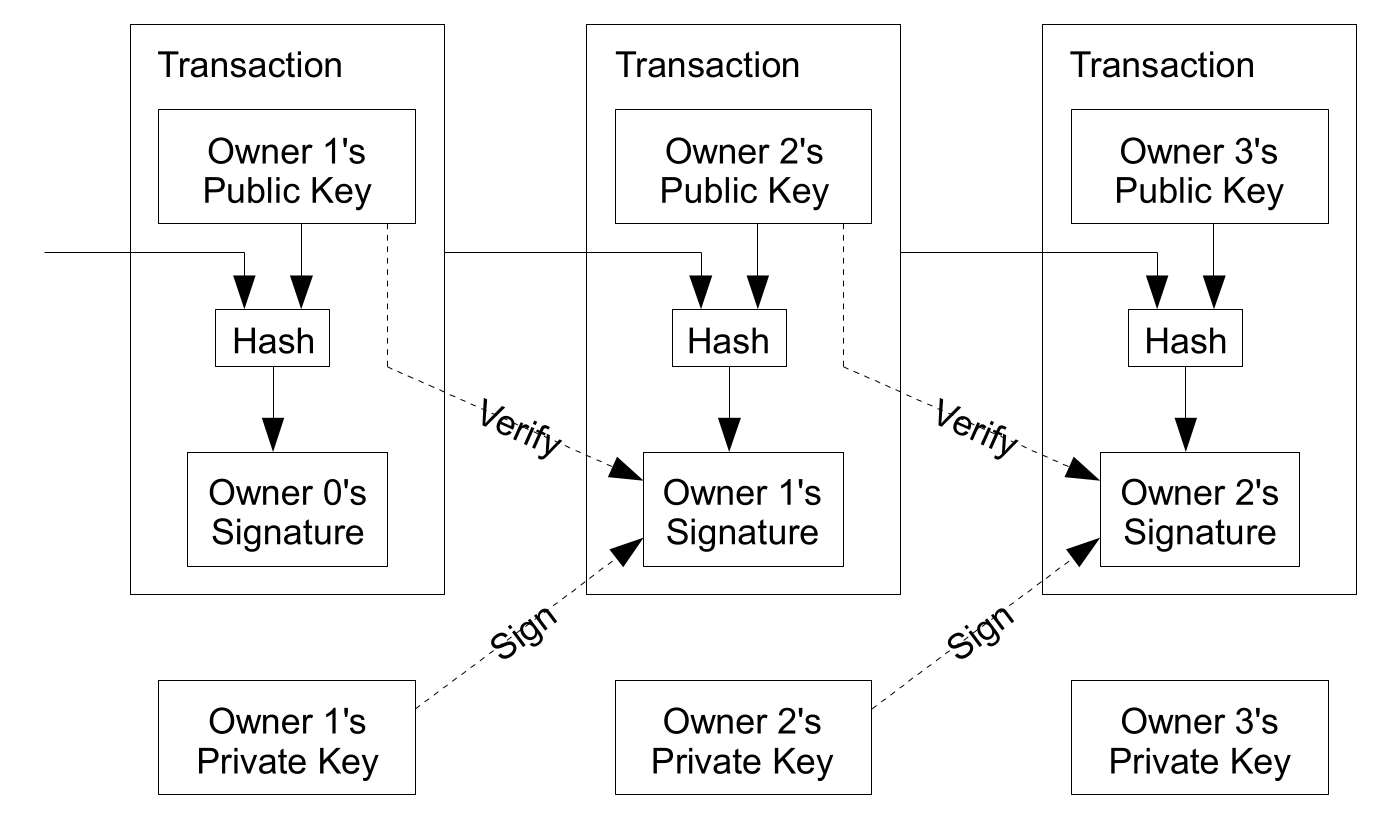
\includegraphics[width=0.8\columnwidth]{figures/bitcoin-tx}
    \caption[Bitcoin coin ownership transfer]{Transfer of ownership signature chain, from~\cite{nakamoto2008bitcoin}}
    \label{fig:bitcoin-tx}
\end{figure}

This ensures that, as long as a participants sign transactions at most once:
\begin{itemize}
    \item By verifying the chain of signatures, every participant can verify which participant owns which coin
    \item Only the owner of a coin can initiate a transaction with that coin
\end{itemize}

Bitcoin enforces that participants can only sign transactions once thanks to its proof-of-work
(see~\ref{subsec:btc:pow}) algorithm.

\subsection{Proof-Of-Work}\label{subsec:btc:pow}

Bitcoin ensures 'unique signatures' in transactions by grouping transactions in immutable, public \textit{blocks}.
Participants can then verify a payer has not signed a hash of a single transaction twice by looking at all existing
transactions.\\

Blocks are made immutable by including in them a value (called a \textit{nonce}) and the hash of the previous block.
% TODO verify it is the hash of the entire block that must yield the zeroes (implementation detail really)
The protocol then accepts only blocks where the $n$ first bits of its hash are zeroes. \\

Thus, in order to publish a block a participant must do work to find a nonce such that the block's hash meets this
condition - then other participants can verify its validity with a single hash operation.
This guarantees that a block cannot be changed (ie, a new copy published) without redoing the computational work.
Because blocks are chained (they include the hash of the previous block), in order to modify a transaction in the past
an adversary needs to redo the computational work for every block since that transaction (see Figure
\ref{fig:bitcoin-blockchain}).
% TODO implementation of mining rewards
Additionally, participants that successfully find a suitable nonce and propose new blocks (also referred to as
\textit{miners}) are allowed to add a specific transaction to the block where they own a newly created coin (also
referred to as \textit{mining reward}).

\begin{figure}[th]
    \centering
    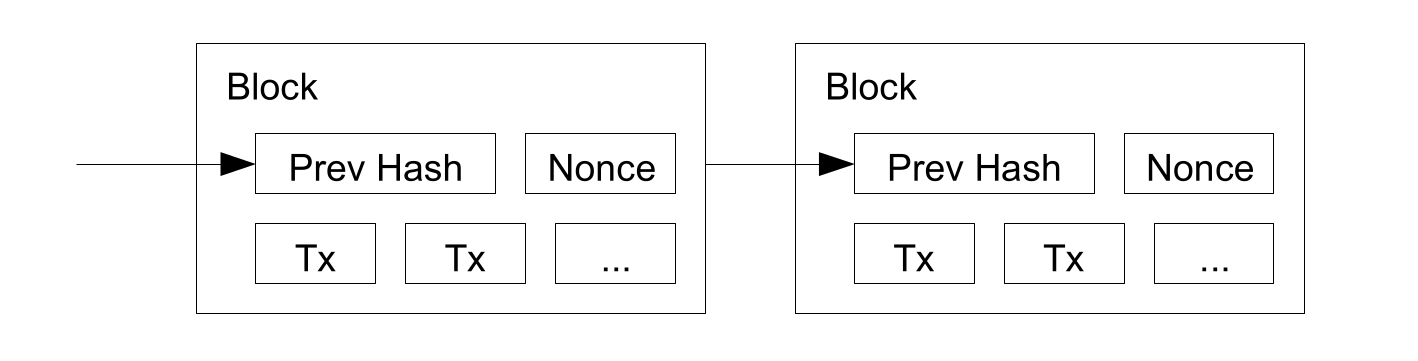
\includegraphics[width=0.8\columnwidth]{figures/bitcoin-blockchain}
    \caption[Two last blocks in a blockhain]{Two last blocks in a blockchain, from~\cite{nakamoto2008bitcoin}}
    \label{fig:bitcoin-blockchain}
\end{figure}

This model of consensus ensures that
\begin{itemize}
    \item Participants have a monetary incentive to stay honest with respect to the protocol
    \item An honest chain will out-compete an adversary's chain as long as the majority of computing power is honest
\end{itemize}

\subsection{Further details of the Bitcoin protocol}\label{subsec:btc.details}
\begin{figure}[th]
    \centering
    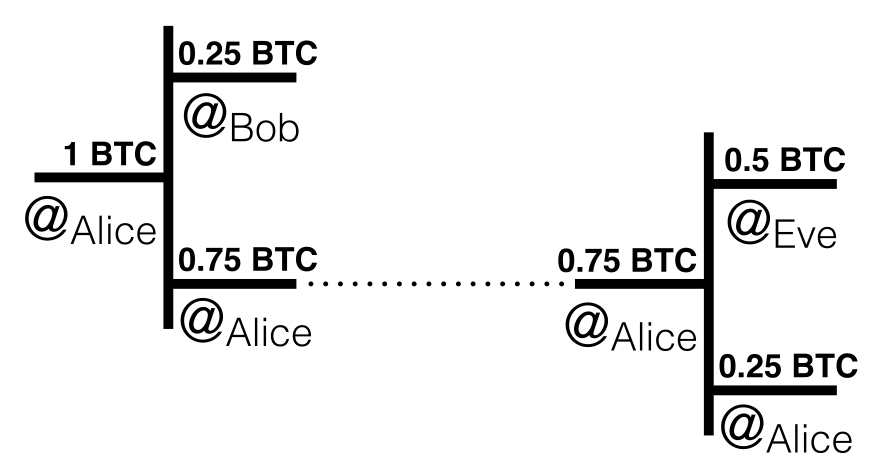
\includegraphics[width=0.6\columnwidth]{figures/bitcoin-2txs-outputs}
    \caption[Outputs and Inputs of two consecutive Transactions]{The outputs of a transaction correspond to
    the input of the next transaction (miner's fee not represented) from~\cite{gervais2022distribLedgers_transactionsInBitcoin}}
    \label{fig:bitcoin-2txs-outputs}
\end{figure}

While I provide a high-level overview of what makes the protocol function, there are many more details that combined
allow for more efficiency and usability:
\begin{itemize}
    \item Transactions may have several inputs and outputs, so participants can transfer amounts rather than single
    \textit{electronic coins}.
    When performing a payment, a typical transaction by Alice has two outputs: the amount she is paying Bob and the
    remainder, which makes up the rest of her funds (see Figure~\ref{fig:bitcoin-2txs-outputs}).
    Thus, a participant's balance is the sum of all the unspent outputs of previous transactions (the set of unspent
    outputs is commonly called the \textit{UTXO} set).
    \item By modifying how many of the leading bits of a blocks' hash must be zeroes, the average computation necessary
    to produce a new block can be adjusted by the protocol.
    \item By using Merkle Trees~\cite{merkle1980tree} transactions with fully spent transaction outputs can be discarded
    without breaking the block's hash.
    This allows compacting old blocks to reclaim disk space.
    \item A participant that does not wish to mine or hold a copy of the entire blockchain can still verify payments.
    It can keep a copy of the block headers of the longest chain and link a transaction to where it is on-chain and
    check that other network nodes have accepted it.
    This process is called \textit{Simple Payment Verification} (SPV)~\cite{nakamoto2008bitcoin}.
    \item Miners have an additional incentive (other than the mining reward) to verify transactions: the
    \textit{transaction fee}.
    The difference of the sum of a transaction's inputs and the sum its outputs corresponds to the transaction fee, which
    goes to the miner.
    \[
        \text{fee}_\text{miner} = \sum{\text{inputs}} - \sum{\text{outputs}}
    \]
    This provides an incentive for the miner to place this specific transaction in the block they propose.
\end{itemize}
\\

For more information on all the workings of the Bitcoin protocol, please refer to~\cite{nakamoto2008bitcoin}.


\section{Smart Contracts and Ethereum}\label{sec:ethereum}

Smart contracts~\cite{szabo1997smart-contracts}, where a protocol formalises a secure agreement or program over a
network, are supported to some extent in Bitcoin (see~\ref{sec:bitcoin}) through scripting~\cite{bitcoinwiki-scripts}.

A bitcoin script is a list of instructions in the \textit{Script} language recorded with each transaction
(see~\nameref{subsec:btc:txs}) that gets executed by every participant that verifies that block and describes how the
payee can access the coins being transferred.
Bitcoin's Script has several limitations, such as lack of Turing-completeness (not all computable functions can be
represented in Script), value blindness (a script cannot easily specify an exact amount to be
withdrawn) and lack of internal state (beyond whether a transaction output is spent or
unspent)~\cite{buterin2015ethereum}.\\

Ethereum is also a blockchain sharing many of Bitcoin's features, such as transactions and
a proof-of-work consensus algorithm.
While it also as scripting support, it varies greatly from Bitcoin's in that its built-in programming language is
Turing-complete, value-aware and allows keeping internal state.
For more details on Ethereum's scripting language, see~\ref{subsec:eth:contract_langs}.
The name of the coin of the Ethereum Ecosystem is \textit{ether}.

Ethereum's state is encoded in \textit{accounts} - objects with their own address that contain the account's
balance~(in ether), the contract code~(if present), the nonce~(a transaction counter), and the account's
storage~(a persistent key-value store which is initially empty)~\cite{buterin2015ethereum}.\\

% TODO talk about eth state transitions (slides from distrib are good) if we'll be using eth

\subsection{The Ethereum Virtual Machine}\label{subsec:eth:contract_langs}

Ethereum's built-in scripting language is a stack-based low-level bytecode language called \textit{EVM language},
and runs on an execution environment called the \textit{Ethereum Virtual Machine} (EVM).
Besides its stack, the EVM does have memory (an infinitely expandable byte array) which resets after each computation.
For persisting data, the account's storage is used~\cite{buterin2015ethereum}. \\

There are several high level languages that compile to EVM bytecode that are used to write smart contracts, such as
Solidity~\cite{solidity_repo} and Vyper~\cite{vyper_repo}~(the most active and maintained languages at the
time of writing~\cite{eth_smartContractLangs}).

% TODO code an examples if you're going to be writing on these

An application built on top of decentralised smart contracts is commonly called a \textit{Decentralised Application} (or
DApp)~\cite{masteringEthGlossary}.

\subsection{Gas Fees in Eterum}\label{subsec:eth:gas}

When performing a transaction, an Ethereum account pays transaction fees (similarly to bitcoin as explained
in~\ref{subsec:btc.details}) from their balance.
Computational steps when scripting are priced in units of \textit{gas} (most commonly, a step costs 1 gas).
When performing a transaction, the sender specifies the values \texttt{STARTGAS} (the maximum amount of gas they are
willing to spend in the transaction execution) and \texttt{GASPRICE} (the price of a single gas unit in ether).\\

Therefore, when executing a smart contract its cost (the fee to be paid for its execution, in ether) will be determined
by the computation it requires (more computation means more gas!).
It is in the interest of the caller of the contract that the contract requires as little computation as possible, so
that the fee they pay for the call remains low.

%TODO should I extend? It is so much shorter than bitcoin


\section{Zero-Knowledge Proofs}\label{sec:zero-knowledge-proofs}

An \textit{Interactive Proof} is a protocol where a verifier $V$ either \textit{accepts} or \textit{rejects} whether a
prover $P$ knows something~\cite{damgaard1998zk_protocols}.
For example, $P$ could be trying to convince $V$ that they know the preimage of a hash.

An interactive proof system has two key properties~\cite{smart2016zeroknowledgeproofs}:
\begin{description}
    \item[Completeness] If $P$ knows the thing being proved and follows the protocol, then $V$ should accept with
    probability one.
    \item[Soundness] If $P$ does not know the thing being proved, then $V$ should only have a negligible probability of
    accepting.
\end{description}

A \textit{Zero-Knowledge Proof} is an interactive proof with the additional property of \textit{zero-knowledge}, where
$V$ accepts without having learned any new information during their exchange with $P$~\cite{damgaard1998zk_protocols,
    smart2016zeroknowledgeproofs}.
In our example, a zero-knowledge proof where $P$ convinces $V$ that they know the preimage of a hash would require $P$
not sharing any information about (or related to) the preimage itself.

This protocol has the interesting property that the information $P$ has proven to know is still private to $V$, and
$V$ is unable to reproduce the proof and convince a third party (say, $V'$) that they (or $P$) know that information.

\subsection{Zero-Knowledge Succinct Arguments of Knowledge (zkSNARKs)}\label{subsec:zksnarks}

% TODO do I need to go through eliptic curve math :c

Interactive proofs assume the prover is computationally unbounded (and so worries about computationally
unbounded adversaries), but by relaxing the soundness property to computationally sound proofs we can assume a
polynomial time prover~\cite{damgaard1998zk_protocols}.

This variation of an interactive proof is called an \textit{interactive argument} (because an unbounded adversary would
be able to fool $V$)~\cite{smart2016zeroknowledgeproofs}.

If we also preserve the zero-knowledge property, we have a \textit{zero-knowledge argument}, which can now be
efficient because it can run in polynomial time~\cite{naranker2022zeroknowledge}.

Additionally, if the prover is unable to construct a proof without some sort of secret (in our previous example, the
preimage of a hash function), then we have an argument \textit{of knowledge}.
Intuitively, in a zero-knowledge argument of knowledge, $V$ becomes convinced that $P$ knows some secret without the
protocol leaking any information about the secret.\\

If our zero-knowledge argument of knowledge additionally satisfies the properties of being \textit{non-interactive}~(no
or little interaction between prover and verifier) and \textit{succinct}~(the sizes of the messages are small in
comparison to the length of the actual computation), then we have a \textit{Zero-Knowledge Succinct Argument of
Knowledge} (or \textit{zkSNARK})~\cite{reitwiessner2016zksnarks}.

\subsection{zkSNARKs on Blockchains}\label{subsec:onchain-snarks}

Recent applications of zkSNARKs include privacy preserving blockchains (see~\ref{sec:bitcoin}) where a network can
verify a participant does not spend more funds that their balance without leaking any knowledge about the amount being
spent, the balance itself, or the identities of payer and payee~\cite{zerocash_whitepaper}.\\

% TODO would be nice to talk about ETH costs which are so so high
Complex smart contracts (see~\ref{sec:ethereum}) quickly result in high costs for callers due to gas costs that increase with complexity of the
contract's computation (see~\nameref{subsec:eth:gas}).
zkSNARKs allow to verify a computation for a fraction of the cost of running it~\cite{zokrates_intro}.

% TODO cite other frameworks?
Several frameworks allow writing zkSNARKs and deploying them to a blockchain that supports smart contracts.\\

\textit{ZoKrates}~\cite{zokrates_repo} allows writing off-chain programs (which can be run tested locally) for a
verifier.
The programs can also be exported as Solidity programs~(see~\ref{subsec:eth:contract_langs})~\cite{solidity_repo} which
can then be deployed to the Ethereum network.
%TODO zokrates 1.6m gas ouch

% TODO STARKS??


\section{Licensing}\label{sec:licensing}

A legal agreement is a fairly broad definition wich varies with each country's legal system.
Most generally, it involves~\cite{contractDef2018precedent}:
\begin{itemize}
    \item An offer by a party
    \item An acceptance by another party
    \item Intention to create a legal relationship
    \item Consideration for the offer - a sort of `promise' where a price is paid for the offer (monetary or
    otherwise).
\end{itemize}

A licence is a specific kind of legal agreement which allows a party to perform an activity under some specific
conditions\cite{licenseDefinition}.
In order to limit the scope, this project will only consider licences (rather than legal agreements as a whole).

\subsection{Dataset Licensing}\label{subsec:licensing:dataset}

\subsection{Software Licensing}\label{subsec:licensing:software}
See~\cite{jetbrainsEduLicense} for an example of a software license between a software company (JetBrains) and users for
the use of their development software.
The license includes the following clauses, cherry-picked and simplified here for clarity:
\begin{itemize}
    \item The software must be used only for specific but vague purposes \textcite[for non-commercial, educational purposes
    only]{jetbrainsEduLicense}.
    \item Only the licensee is allowed to use the software, but they may install it in multiple machines simultaneously.
    \item The software cannot be sold, rented, or modified.
    \item The licensee may provide feedback - if they choose to do they themselves grant JetBrains a very permissive
    license to use it.
    \item There is a number of exceptions where JetBrains can revoke access - but in general, they may at any point
    terminate the agreement without a specific reason.
    \item The user may choose to use an early access development version of the software, subject ot its own separate
    license.
\end{itemize}

% TODO

    \chapter{A Domain Specific Language for Legal Agreements}\label{ch:lang}

One of the key focuses of this project is not just to be able to represent legal contracts with specific properties and capabilities (as described in~\autoref{ch:queries});
but also to make it as easy as possible for people with non-technical backgrounds to use such representations.
Simply put, a lawyer should not need to learn JSON nor temporal logic.

This is the main motivation for developing tooling which aims to make it easier for people of non-technical backgrounds to produce, modify, and understand Confis legal agreement representations.
The core of this tooling is the Confis language~(\autoref{sec:language-semantics}) and an IDE-assisted editor~(\autoref{sec:confis-editor}).


\section{Motivations For a DSL}\label{sec:dsl-motivations}

\subsection{Implementation Requirements}\label{subsec:dsl:requirements}

The language should fulfil the core requirements set out in~\autoref{sec:objectives}.
This involves prioritising accessibility while making sure the language stays expressive enough.

\subsubsection{Easy to write while still machine-readable}

Writing a Confis agreement should be close to writing natural language, while still being machine-readable.
For more details on the meaning of \emph{machine-readable} in the context of this project, see~\autoref{sec:machine-readable-contracts}.

\paragraph{Data Serialization Language}

On one extreme, a data serialization text file (like JSON, YAML, or XML) would allow writing text that can be easily parsed by a program.
But writing such files requires some data structures knowledge;
and because of their key-value nature they do not allow writing sentences, leaving them too far from the readability of human-written legal prose -- thus they lack they are not accessible.

\paragraph{Natural Language Processing}

On the other extreme, legal prose processed through a language processing program allows the drafter to completely ignore the machine-readable aspect of the document.
Readers would be able to integrate such documents in their existing workflows -- as they would need to make no transition from their existing, non-machine-readable documents.
This is approach is discussed in~\autoref{sec:nlp} -- we conclude it does not meet the expressiveness property faithfully enough, since it cannot specify contracts accurately.

A compromise between these two solutions would be a language formal enough that it can be parsed by a program, but natural enough that natural language sentences can be recognised in it.
Python or AppleScript~\cite{Sanderson2010appleScript}~(see~\autoref{fig:appleScript}) are good examples of programming languages (and therefore parseable) that are engineered with the goal of resembling English as much as possible.

\begin{listing}[h]
    \centering
    \begin{minipage}{0.7\textwidth}
        \begin{minted}[
            autogobble,
            frame=lines,
            framesep=2mm,
            fontsize=\small
        ]{applescript}
                set the firstnumber to 1
                set the secondnumber to 2
                if the firstnumber is equal to the secondnumber then
                    set the sum to 5
                end if
        \end{minted}
    \end{minipage}
    \caption{Sample code snippet of the AppleScript Language~\cite{Sanderson2010appleScript}}
    \label{fig:appleScript}
\end{listing}

\paragraph{Easy to develop and extend}

With pragmatic implementation efforts in mind, this project should not aim to develop its own parser and interpreter or compiler: the project hopes to be more concerned with introducing a suitable abstraction that allows specifying legal documents.

\paragraph{Additional tooling for ease of use and correctness}

A key aspect of development for a new user of a language is to understand the concepts of syntax, compile errors, and invalid programs.
A great aid to developing this understanding are visual cues in editors in integrated development environments (or IDEs).

For the Confis DSL to be successful, it must be easy for the drafter of legal agreements to reason about the correctness of the document within the formalisms set out by this project.
Good tooling is therefore a key requirement in order to achieve accessibility, a key priority as discussed in~\autoref{sec:objectives}.

\subsection{Implementation Requirements Conclusion}\label{subsec:dsl-design-conclusion}

The requirements of~\autoref{subsec:dsl:requirements} lead to the following design choices:

\paragraph{A Textual Domain-Specific Language} For a good compromise between readability, flexibility and rigidity of the agreements that can be written, this project therefore proposes developing a DSL~(see~\nameref{sec:dsls}) as a suitable compromise that allows working with a human-readable encoding which can then be compiled to a suitable machine-readable representation.

We will call this language \textbf{\emph{Confis DSL}} (or \emph{Confis language}) and the machine-readable representation it compiles to \textbf{\emph{Confis Internal Representation}} (or \emph{Confis IR}).
The Confis IR will be used for processing as discussed in~\autoref{ch:queries}.

\paragraph{An Internal DSL}
For the sake of development costs, we use a suitable host language to implement the Confis DSL (as opposed to developing an external DSL).
The alternative (developing an entirely new language) is discussed in~\autoref{sec:future-work}.

\paragraph{Kotlin as a host language} Several host languages can serve to build a DSL.
A few options are discussed in~\autoref{subsec:dsl-host-candidates}, like Groovy and Haskell.
The choice to use Kotlin stems from how feature-rich the surrounding tooling is -- such as its stand-alone custom scripting~\cite{kotlinScriptKeep} and IDE support~\cite{intelliJRepo}.


\section{Language Semantics and Design}\label{sec:language-semantics}

This section is concerned with the structure, semantics, and design decisions regarding the Confis DSL.
For the implementations details of the DSL, see~\nameref{subsec:dsl-implementation}.

As described in~\autoref{sec:objectives}, both accessibility and expressiveness are key priorities in designing the language.
Confis introduces the following formalisms in order to limit the complexity of the language.
These definitions make up the internal representation (IR) and are used to later generate rules to effectively answer complex queries.
The language is designed to easily specify these abstractions.
Therefore, this project tries to keep abstractions simple and introduce as few and as simple of them as possible, in order to design a parsimonious language.

\begin{definition}[Party]
    \label{def:party}

    A \emph{Party} to the agreement is a legal person (a real person, an institution, a company, or even a group of people).
    Parties are unique in an agreement and are identifiable by a name (encoded as a UTF-8 string).
\end{definition}

\begin{definition}[Action]
    \label{def:action}
    An \emph{Action} represents something that can be initiated by a Party.
    It is unique in an agreement and is identifiable by a name (encoded as a UTF-8 string).
\end{definition}

\begin{definition}[Thing]
    \label{def:thing}
    A \emph{Thing} is unique in an agreement and is identifiable by a name (encoded as a UTF-8 string).
    An Thing resembles a~\nameref{def:party} but it does not aim to represent a legal person and it cannot be a subject on a~\nameref{def:sentence}.
\end{definition}

A Sentence is the building block of a Confis agreement.
It is combined with other elements in order to form clauses and, combined with a Circumstance Set, it forms an event that includes a context.

\begin{definition}[Sentence]
    \label{def:sentence}
    A \emph{Sentence} is a tuple like~\texttt{Sentence = (Subject, Action, Object)}, where a \texttt{Subject} is a~\nameref{def:party} and \texttt{Object = Party | Thing}.
\end{definition}

Allowance is used to answer questions of the type \emph{`May A do X?'} -- where \emph{yes} or \emph{no} are not enough to model all the possibilities given in the legal domain.


\begin{definition}[Allowance]
    \label{def:allowance}
    \emph{Allowance} is a value like \texttt{Allowance = Allow | Forbid | Unspecified | Depends}.
\end{definition}

Users are allowed to use Allowance in order to define a~\nameref{def:permission}, but only with the values \texttt{Allow} and \texttt{Forbid}.
The other values are reserved for answering queries and while they cannot be used, responses that return \texttt{Depends} and \texttt{Unspecified} can be crafted by defining the answer space accordingly.
This is shown in~\autoref{fig:allowance-venn} and~\autoref{eq:allowance-cake-example}, where only \texttt{may} and \texttt{mayNot} keywords are used (corresponding to \texttt{Allow} and \texttt{Forbid} respectively) but all possible values of Allowance are present in the agreement.

\begin{listing}[h]
    \centering
    \begin{minipage}{0.5\textwidth}
        \begin{minted}[
            autogobble,
            fontsize=\small,
%            frame=lines,
%            framesep=2mm
        ]{kotlin}
            val alice by party
            val eat by action
            val cake by thing

            alice may eat(cake) asLongAs {
                with purpose Research
            }
            alice mayNot eat(cake) asLongAs {
                with purpose Commercial
            }
        \end{minted}
    \end{minipage}
    \caption{Minimal 2-clause agreement with disjoint Permissions}
    \label{list:disjoint-confis}

\end{listing}


\begin{figure}[h]

    \centering
    \begin{tikzpicture}
        \node [
%        draw,
        circle,
        fill=gray,
        minimum size =5cm,
        label={135:$\text{alice eat cake}$}] (Eat) at (1.25,0){};

        \node [
%        draw,
        circle,
        fill=mdtGreen,
        minimum size =2.5cm,
        label={180:$\text{\small with purpose Research}$}] (A) at (0,0){};

        \node [
%        draw,
        circle,
        fill=mdtRed,
        minimum size =2.5cm,
        label={0:$\text{\small with purpose Commercial}$}] (B) at (2.5,0){};

        \node[white] at (0, 0) {\texttt{Allow}};
        \node[white] at (2.5, 0) {\texttt{Forbid}};
        \node[white] at (1.25, 1.5) {\texttt{Depends}};
        \node at (5, 1.5) {\texttt{Unspecified}};

    \end{tikzpicture}

    \caption[Venn diagram of query for disjoint circumstances agreement]
    {Venn Diagram of a `\texttt{alice eat cake}?' query for~\autoref{list:disjoint-confis}}
    \label{fig:allowance-venn}
\end{figure}

\begin{align}
    \label{eq:allowance-cake-example}
    \text{alice eat cake?} &\to \texttt{Depends}\\
    \text{alice eat cake with purpose Research?} &\to \texttt{Allow}\\
    \text{alice eat cake with purpose Commercial?} &\to \texttt{Forbid}\\
    \text{alice eat cake with purpose Internal?} &\to \texttt{Unspecified}
\end{align}


\begin{definition}[Permission]
    \label{def:permission} A \emph{Permission} represents a legal capability (or lack thereof) in the language.
    It is a tuple of a~\nameref{def:sentence}, an~\nameref{def:allowance}, and a~\nameref{def:circumstanceSet} (which may be empty).
    \begin{verbatim}
        Permission = (Sentence, Allowance, CircumstanceSet)
    \end{verbatim}
\end{definition}

A requirement is an important abstraction necessary in order to define~\nameref{def:confis-compliance}.
Confis also assumes a that providing a legal obligation entails providing the legal capability to fulfill that obligation, which means that when we have a Requirement we have an \texttt{Allow} Permission too.

\begin{definition}[Requirement]
    \label{def:requirement} A \emph{Requirement} represents a legal obligation and is a tuple of a~\nameref{def:sentence} and a~\nameref{def:circumstanceSet} (which may be empty).
    \begin{verbatim}
        Requirement = (Sentence, CircumstanceSet)
    \end{verbatim}

    A requirement $r$ entails a permission $p$ where if $r = (s, C)$ then $p = (\texttt{Allow}, s, C)$
\end{definition}

\begin{definition}[Event]
    \label{def:event}
    An \emph{Event} is a tuple of a Sentence and a Circumstance set, describing the context the Sentence happens in, like \texttt{Event = (Sentence, CircumstanceSet)}
\end{definition}

We use a set of Events to represent a `state-of-the-world'.
Note how we have no concept of precedence or ordering between events.
The only way to order chronologically them would be with respect to a time-based Circumstance present in each event's Circumstance Set.

\begin{definition}[Compliance]
    \label{def:confis-compliance}
    We say that a Requirement $r$ \emph{has been met by} a set of Events $W$ if and only if there is an event $e \in W$ such that they have the same Sentence and the Circumstance Set of $e$ is generalised by the Circumstance Set of $r$.

    We say that a \texttt{Forbid} Permission $p$ \emph{is respected by} a set of Events $W$ if and only if there does not exist $e \in W$ such that $e$ has the same Sentence as $p$ and the Circumstance Set of $e$ overlaps with the Circumstance Set of $p$.

    A set of Events $W$ \emph{is compliant with} an agreement if and only if, for every Requirement $r$ and every \texttt{Forbid} Permission $p$ that are part of the agreement, $r$ has been met by $W$ and $p$ is respected by $W$.
\end{definition}

For the meanings of `generalises' and `overlaps with', see~\autoref{def:circumstanceSet:generalise}, and~\autoref{def:circumstanceSet:overlap}.

\subsection{Circumstance and Circumstance Set}\label{subsec:circumstance}

Circumstances are a core abstraction in Confis, both in the language and in~\nameref{sec:rule-generation} (hence why they deserve their own section).

A Circumstance Set represents the context in which a~\nameref{def:sentence} may occur.
In the context of a legal agreement, it would contain everything in a clause that is not the core sentence, including the parent clause, conditions, etc.

A Circumstance Set is made up of Circumstances.


\begin{definition}[Circumstance]
    \label{def:circumstance}
    $c$ is a \emph{Circumstance} if and only if it is equipped with the following operations for any other circumstance $c'$:
    \begin{align}
        \label{def:c:generalise}
        \texttt{generalise}&: \ c \to\ c' \to\ \texttt{Boolean}\\
        \label{def:c:provideKey}
        \texttt{provideKey}&: \ c \to\ k\\
        \label{def:c:overlap}
        \texttt{overlapsWith}&:\ c \to\ c' \to\ \texttt{Boolean}\\
        \label{def:c:render}
        \texttt{render}&: \ c \to\ \texttt{String}
    \end{align}
\end{definition}

A circumstance key $k$ is simply an element with a notion of equality.
When two circumstances $c_1$ and $c_2$ produce they same key $k$, they are said to be~\emph{of the same type}.
\texttt{render} is a function made to satisfy the requirement of being able to convert a Confis agreement into readable English for the sake of accessibility, and necessary to display query results in natural language.

A Circumstance Set is an indexed set of~\nameref{def:circumstance}s, unique in that only one circumstance of each type can be stored.
For example, we can only store a single circumstance representing time and a single circumstance representing purpose, because these are implemented to produce the same key $k$ each.

\begin{definition}[Circumstance Set]
    \label{def:circumstanceSet}
    A \emph{Circumstance Set} is a key-value mapping of Circumstance Keys to \nameref{def:circumstance}, like $\texttt{CircumstanceSet} = \{ k \to \texttt{Circumstance} \}$.
\end{definition}

Defining a \texttt{generalise} equivalent for circumstances will be of use when trying to define rules (see~\autoref{sec:rule-generation}) because it will allow checking whether a circumstance from a clause `matches' that of a question~(see~\nameref{subsubsec:circumstances-intuition} for an explanation).

\begin{definition}[Circumstance Set Generalisation]
    \label{def:circumstanceSet:generalise}
    Fot two Circumstance Sets $C_1$ and $C_2$ we say $C_1$ \emph{generalises} $C_2$ if and only if:
    \begin{equation}
        \label{eq:circumstanceSet:generalisation}
        \forall k \, \forall c_1.[ \, (k, c_1) \in C_1 \to
        \exists c_2.((k, c_2) \in C_2  \land\ c_1\ \texttt{generalises}\ c_2)\,]
    \end{equation}

    That is, if for all circumstances in $C_1$, there is a circumstance of the same type in $C_2$ and each circumstance in $C_1$ generalises the circumstance of the same type in $C_2$.
\end{definition}

\begin{definition}[Circumstance Set Overlap]
    \label{def:circumstanceSet:overlap}
    For any two Circumstance Sets $C_1$ and $C_2$, we say $C_1$ \emph{overlaps with} $C_1$ if and only if
    \begin{equation}
        \label{eq:circumstanceSet:overlap}
        \forall k \, \forall c_1.[ \, (k, c_1) \in C_1 \to
        \exists c_2.((k, c_2) \in C_2  \land\ c_1\ \texttt{overlapsWith}\ c_2)\,]
    \end{equation}
    That is, if for all circumstances in $C_1$, there is a circumstance of the same type in $C_2$ and each circumstance in $C_1$ overlaps with the circumstance of the same type in $C_2$.
\end{definition}

This definitions of Circumstance Set Generalisation and Overlap have the following consequences:
\begin{itemize}
    \item The empty circumstance set generalises all circumstance sets
    \item The empty circumstance set overlaps with all circumstance sets
\end{itemize}


Although nothing requires Circumstance Set overlap to be commutative, it will be commutative if the Circumstances it contains have a commutative implementation of \texttt{overlapsWith}.
This is the case for every Circumstance built into Confis so far.

\subsubsection{Intuition Behind Circumstances}\label{subsubsec:circumstances-intuition}

Circumstance Sets can be thought of as contexts for a sentence, which together constitute an event.
Defining overlaps and generalisations between these contexts allows us to reason about the same concepts for events: is \emph{`Pay Bob during the month of June'} more general than \emph{`Pay Bob the 10th of June'}? Defining a time range (a day in June, a month within a year) as a Circumstance allows us to answer those questions programmatically.

The empty circumstance set can be thought of as the least specific context for an event (think of it as \emph{anywhere} when thinking about a place).
Indeed, the event \emph{`Alice pays Bob'} generalises the event \emph{`Alice pays Bob during June'}.
If a contract has a requirement for the former, and we supply it with a state of the world containing the latter, we can say that Alice is compliant with the contract!

Likewise, the converse is true for \emph{disjoint} (not overlapping) events.

For two events $e_1 = \textit{`Alice pays Bob during June'}$,  $e_2 = \textit{`Alice pays Bob during September'}$, we can say the Circumstance Sets of $e_1$ and $e_2$ are disjoint, therefore if a contract requires $e_1$ but we have a state of the world with $e_2$, we can say Alice still has some legal obligation she has not fulfilled.

Generally, Circumstance Sets describe more specific situations the more elements they have.
How different Circumstance Sets can overlap and generalise each other is shown by example through the definitions of the sets $A$, $B$, $C$, $D$ and $E$ below.

\begin{align}
    A &= \{ \texttt{time} \to \text{`10th of June 2022 - 12th of June 2022'} \}\\
    B &= \{ \texttt{time} \to \text{`1st of June 2022 - 31st of June 2022'} \}\\
    C &= \{ \texttt{purpose} \to \text{`Commercial'} \}\\
    D &= A \cup C\\
    E &= \{ \texttt{time} \to \text{`1st of June 2022 - 11th of June 2022'} \}
\end{align}

% TODO this is wrong fix it
We have:
\begin{itemize}
    \item The empty Circumstance Set $\emptyset$ generalises and overlaps with $A$, $B$, $C$, $D$ and $E$
    \item $B$ generalises $A$ and $E$
    \item $A$ overlaps with $B$, $D$ and $E$
    \item $B$ overlaps with $A$, $D$ and $E$.
    \item $D$ overlaps with $A$, $B$, $C$, and $E$.
    \item $E$ overlaps with $B$, $D$ and $A$
    \item $C$ overlaps with $D$
\end{itemize}

\subsection{DSL Implementation}\label{subsec:dsl-implementation}

This subsection is concerned with the implementation details of the Confis DSL.
For design decisions regarding the language (like what is a Sentence or the difference between a Requirement and a Capability) please see~\nameref{sec:language-semantics}.

Because of the nature of internal DSLs~(see~\autoref{sec:dsls}), the syntax of the Confis DSL must be a subset of the Kotlin language's.
% TODO add future work link for own lang
Given the Confis DSL and the Confis IR are decoupled this section will not go into too much detail on how the DSL is implemented as most of that is specific to the Kotlin language, and the DSL could have been implemented as an internal DSL with a different host language anyway (like Haskell or Groovy).
Instead, it will show a couple examples of how language constructs are implemented (like a Permission) which will be useful to understand~\autoref{subsec:editor-implementation}.

For more information on how DSLs can be built in Kotlin in general, see~\autoref{subsubsec:kotlinLang}, and in particular refer to~\cite{kotlinTypeSafeBuilders}.

\subsubsection{Permission Builder Implementation}

Recall a~\nameref{def:permission} is a tuple of~\texttt{(Allowance, Sentence, CircumstanceSet)}, where the \texttt{CircumstanceSet} may be empty.
For the sake of brevity, we will leave the construction of the Circumstance Set out and discuss how we can construct a tuple of \texttt{(Allowance, Sentence)} in the DSL.
% TODO CircumstanceMap
First, we must define the tuple for~\nameref{def:sentence} in Kotlin as in~\autoref{fig:kotlinSentence}.
Recall a \texttt{Sentence} is simply a tuple of \texttt{(Subject, Action, Object)}.

\begin{listing}[h]
    \centering
    \begin{minipage}{0.4\textwidth}
        \begin{minted}[
            autogobble,
            frame=lines,
            framesep=2mm]{kotlin}
        data class Sentence(
            val subject: Subject,
            val action: Action,
            val obj: Object,
        )
        \end{minted}
    \end{minipage}
    \caption{\texttt{Sentence} tuple declaration}\label{fig:kotlinSentence}
\end{listing}

We now need a DSL to construct this \texttt{Sentence}.
We use an infix extension function in order to add the \texttt{`may'} adverb (which corresponds to \texttt{Allowance = Allow}) between the subject and the action of the sentence.
We also use a Kotlin operator function~\cite{kotlinInvokeOperator} in order to overload the \texttt{Action}, so the user is able to write \texttt{action(object)} as opposed to \texttt{ActionObj(action, obj)}.
The full example is demonstrated in~\autoref{fig:permissionKotlinFull}, and a usage example is given in~\autoref{fig:finalPermissionInvocationDSL} -- which reads like an English sentence!



\begin{listing}[h]
    \centering
    \begin{minipage}{\textwidth}
        \begin{minted}[
            autogobble,
            frame=lines,
            mathescape,
            framesep=2mm]{kotlin}
            // <Action, Object> tuple declaration
            data class ActionObject(val action: Action, val obj: Object)

            // this easily builds an ActionObject
            // action.invoke(obj) == action(obj)
            operator fun Action.invoke(obj: Object) = ActionObj(this, obj)

            infix fun Subject.may(s: ActionObject) {
                val permission = Permission(Allow, Sentence(this, s.action, s.obj))
                clauses += permission
            }
        \end{minted}
    \end{minipage}
    \caption{Finished Permission builder}
    \label{fig:permissionKotlinFull}
\end{listing}



\begin{listing}[h]
    \centering
    \begin{minipage}{0.5\textwidth}
        \begin{minted}[
            autogobble,
            frame=lines,
            framesep=2mm]{kotlin}
            val alice: Subject
            val eat: Action
            val cake: Object

            alice may eat(cake)
        \end{minted}
    \end{minipage}
    \caption{Example of the DSL invocation of the final Permission builder of~\autoref{fig:permissionKotlinFull}}
    \label{fig:finalPermissionInvocationDSL}
\end{listing}

We now can call the function \texttt{may()} in order to create a \texttt{Permission} and add it to \texttt{clauses}.
Most of the Confis DSL is implemented similarly.
An advantage of using a statically typed language for a DSL with well-defined types like in the examples given above means that only semantically correct sentences can be written.
For example, \texttt{`cake may eat(alice)'} produces a compilation error, because \texttt{`cake'} is not a \texttt{Subject}.


% TODO is this worth writing about at all


\section{Additional Tooling: Legal Prose Rendering}\label{sec:additional-tooling:doc-rendering}

In order to comply with the accessibility requirement, it should be possible to generate a traditional document (perhaps in plaintext or PDF format) in natural language.
This generated document should then be usable in place of traditional agreement documents -- for example, a reviewer of an agreement will not need Confis software or to know about the Confis DSL in order to read a copy of the contract.

We will call this feature \textbf{\emph{legal prose rendering}}.

If NLP~(see~\autoref{sec:nlp}) aims to translate traditional human-written legal-prose into a machine-readable format, you can think of legal prose rendering as the inverse process: we go from a machine-readable representation to a more human-readable one.

% TODO

\section[The Confis Editor]{Additional Editing Tooling: the Confis Editor}\label{sec:confis-editor}

One of the key requirements for Confis is accessibility.
In order to achieve this the Confis framework includes an extension to the IntelliJ Development Environment~\cite{intelliJRepo} - the \textbf{\emph{Confis Plugin}}.
Bundled with this plugin is the \textbf{\emph{Confis Editor}}.

The Confis Editor has two main goals:

\paragraph{Providing context-aware aid for authoring agreements} Much like an IDE provides relevant aid to a software engineer (such as reporting compile errors before attempting to compile the program) the Confis Editor should allow an agreement drafter to write in the Confis DSL without needing to deal with command-line utilities or knowing the tooling around Kotlin language.

\paragraph{Providing a human-readable preview of the Confis Agreement}

The Confis Editor should display a document in legal prose, made up from text generated from the Confis agreement (thanks to legal prose rendering~\ref{sec:additional-tooling:doc-rendering}).
This preview should resemble a traditional legal document, and appear side-to-side the code the agreement drafter is writing in order to provide a useful live preview of the contract being authored (much like it is handy to have a PDF preview when drafting TeX documents).

\subsection{Editor Implementation}\label{subsec:editor-implementation}

Two things are required in order to be able to draft single Confis code files inside an IDE:
\begin{enumerate}
    \item It must be possible to write a self-contained, boilerplate-free contract in a single file.
    \item The IDE must perform reporting specific to the Confis DSL when editing this file (as opposed to reporting on the host language, Kotlin).
\end{enumerate}

(1.) is where Kotlin's custom scripting support~\cite{kotlinScriptKeep} is crucial.
See~\nameref{subsec:scripting-support} for a discussion on what is meant by scripting and how it is required for making a stand-alone DSL.

In order to implement writing Confis agreements as stand-alone files, we create a \emph{Kotlin Custom Script definition}~\cite{kotlinScriptKeep}, which essentially contains information that assigns an instance of a class to a script.
By placing DSL builder functions like those introduced in~\autoref{fig:permissionKotlinFull} inside a class (called \texttt{AgreementBuilder}, for example) and assigning an instance of this class to a script, we can let the script author (ie, the Confis agreement author) \textbf{mutate} our class when we evaluate their script.

See~\autoref{fig:agreementBuilderSmall} for an example of such a class, and~\autoref{fig:confis:minimal} for an example of a single script bound to that class.

We can then pass the script definition mentioned above to an extension point present in the IntelliJ API engineered specifically for this purpose~\cite{ideaExtensionPoints, intelliJRepo}.
If we include some additional information (such as a file extension for Confis agreements) IntelliJ will now provide visual hints for Confis Scripts.

\begin{figure}[h]
    \centering
    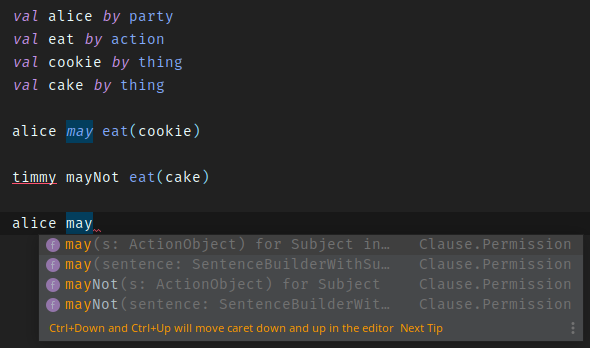
\includegraphics[width=0.75\textwidth]{figures/minimal.editor.highlighting.confis}
    \caption{Syntax highlighting in a small Confis agreement}
    \label{fig:intelliScriptAid}
\end{figure}

See~\autoref{fig:intelliScriptAid} for an example where the Confis editor reports a compile error (where the user attempted to form a Sentence with a Party that does not exist) as well as autocompletion for building a Permission clause.
% TODO actually do this on the website
A live video example can be found in the~\href{https://confis.dcotta.eu/0.1.1/IDE%20Support/IDEAPlugin/}{Confis Documentation Page}.

In order to achieve (2.), we can implement a new editor in IntelliJ based on its existing markdown editor~\cite{ideaMarkdownPreview} which achieves a very similar purpose: providing a live preview of machine-readable code.

The live preview is implemented as a preview of an in-memory Markdown document which is in turn generated upon code changes in the editor:
\begin{equation*}
    \text{Confis Code}\; \to\; \text{Confis IR}\; \to\; \text{Markdown document}\; \to \text{HTML page}\; \to\; \text{Live preview}
\end{equation*}

A screenshot of the Confis Editor, including syntax highlighting and the live preview, can be found in~\autoref{fig:confis.minimal.editor}.

\begin{figure}[h]
    \centering
    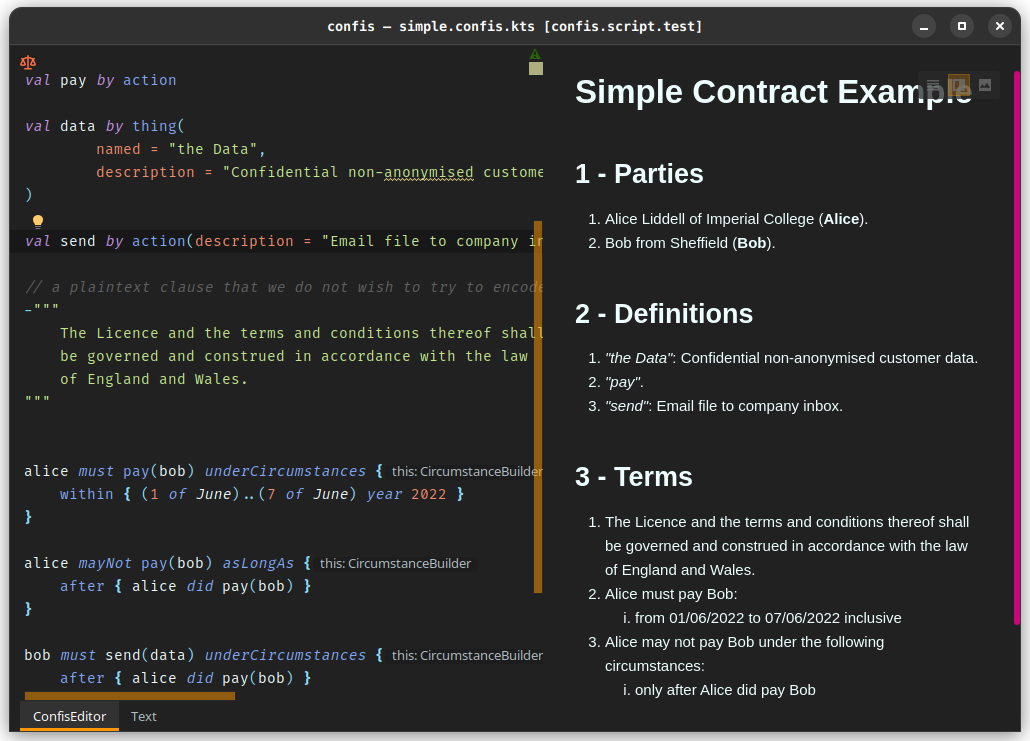
\includegraphics[width=\textwidth]{figures/simple.confis.editor}
    \caption{Screenshot of the Confis Editor, including the legal prose preview}
    \label{fig:confis.minimal.editor}
\end{figure}



For the sake of brevity, this report will omit the implementation details of the live preview -- but a starting point can be found in the software archive under the \texttt{ConfisEditor} class.


\section{Language Documentation}\label{sec:language-documentation}

In the spirit of software engineering principles and to further work towards meeting the accessibility requirement, this project also introduces a documentation website, which can be found at \href{https://confis.dcotta.eu}{\texttt{confis.dcotta.eu}} and is pictured in~\autoref{fig:online-docs}.
It is implemented as a series of Markdown documents rendered as HTML pages thanks to the MkDocs~\cite{mkDocs} tool.

\begin{figure}[h]
    \centering
    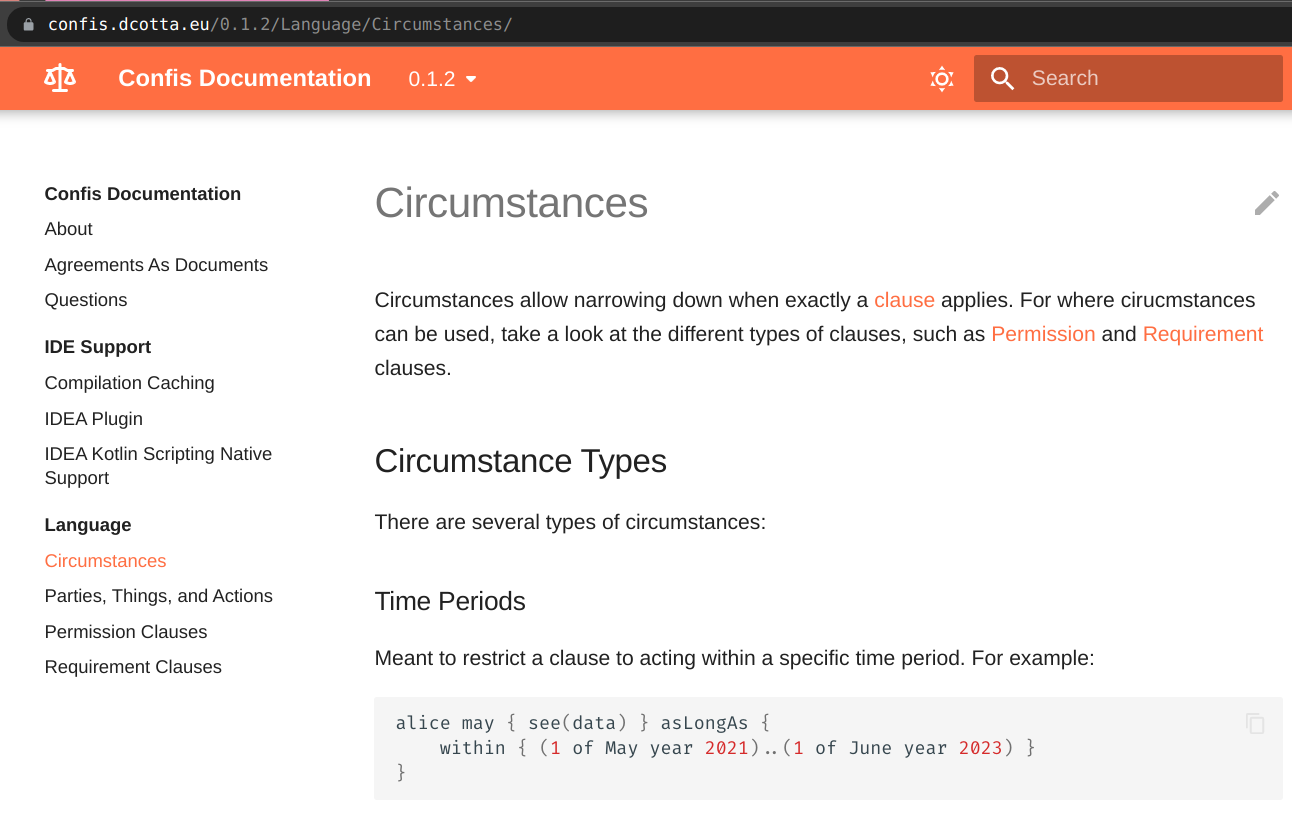
\includegraphics[width=\textwidth]{figures/online-docs}
    \caption{Screenshot of the Circumstances section of the Confis online documentation}
    \label{fig:online-docs}
\end{figure}

The documentation's main aim is to clearly explain~\autoref{sec:language-semantics} without getting into implementation details, nor the specifics of how Circumstances are formalised.



    \chapter{Queryable Documents}\label{ch:queries}

\section{Developing a suitable representation}\label{sec:queries-representation}

\subsection{Requirements}\label{subsec:queries-requirements}

% TODO find a source on why we would want this specifically out of Confis
Assuming an existing document, being able to perform the following operations on said document is desirable: we will call these operations \emph{queries} (or questions) made to the contract.
In order to be accessible, these must be intuitive and should not require deep

% TODO justify this being common
\paragraph{Querying for Legal Capabilities} A common use-case is for a party to want to figure out their legal capabilities with respect to a contract, as well as the capabilities of other parties.
Take the example of a tenancy agreement: a tenant may want to know whether they are allowed to have pets, or whether the landlord is allowed to enter their property.

Therefore, a successful query system should be able to provide answers to questions such as \textit{`May $A$ do $X$?'}

A party may also have some requirements to be able to perform some action - such as performing a payment.
Continuing the example of the tenancy agreement, a landlord may be allowed to enter the premises in case of emergency, but not otherwise.
Thus, a more general question could be `Under what condition may $A$ do $X$?'

\paragraph{Compliance verification} If figuring out a party's legal capabilities is a key part of dealing with a contract, so is figuring out their legal obligations.
Unlike a legal capability question, a compliance question cannot be formulated as \textit{`May $A$ do $X$?'} -- they should instead be along the lines of \textit{`What does X need to do in order to be compliant?'}.
We should also take into account that a party may have already done something to be compliant at the time of performing the query -- therefore we need to include some `state-of-the-world' in our question.
    Additionally, parties usually interact and actions between more than a single party may be needed to achieve compliance.

Therefore, we can generalise a compliance verification question to \textit{`Given a series of past events S, what actions need to take place in order for the contract to be complied with?'}.


\subsubsection{Confis Internal Representation}
As~\cite{knottenbeltContractDriven} notes, there is a clear compromise to be made between how complex a contract representation is, and how simple the computations needed to process it are.

Contrary to solutions discussed in~\autoref{sec:nlp} such as~\cite{sleimi2018NLP4}, Confis does not try to generalise a contract into a set of normative rules (as defined in~\autoref{eq:basic-rule}) straight away.
Instead, it tries to preserve all the information that goes into assembling a contract into an Intermediate Representation (that we will call \textbf{\emph{Confis IR}}).
The Confis IR is then converted into different sets of rules depending on the query being performed.

Therefore, a critical part of Confis is generating rules from the IR.

% TODO examples of DSL -> IR and IR -> rules


\subsection{Tooling for Accessible Queryable Contracts}\label{subsec:tooling-for-accessible-queryable-contracts}

\subsection{Confis as a Generalisation of Ricardian Contracts}\label{subsec:generalisation-of-ricardian-contracts}

    % Chapter Template

\chapter{Ethical Considerations}\label{ch:ethical}

\section{Legal Implications}\label{sec:legal-implications}

 This project hopes to automate enforcement of clauses in legal agreements.
Contracts commonly have exceptions where violating the terms of the agreement is not a breach of the contract in
circumstances outside the control of all parties (referred to as \textit{`Force Majeure'}~\cite{forceMajeureDefinition} -
see~\cite[\textsection13.14]{jetbrainsEduLicence} for an example).\\

% TODO come back to this after writing the intro
It is still to be seen to what extent this project enforces clauses and to what extent it only provides
a decentralised audit trail.
The former may impede actions that could be law-compliant in case of force majeure, while the latter
would give parties more freedom to breach the contract (and leave it up to the other party to follow up with legal
action).

While the latter may seem like a safer option, enforcing compliance outside of courts can be very attractive to all
parties because they would be able to protect the terms of the contract without having to go to court and expending the
financial and legal resources to take action in case of contract breach.
So much so that this is the case already in many software licenses~(where~\cite{jetbrainsEduLicence} is a prime example),
where the end user has their access revoked before the licensor.
% TODO PICKUP talk about existing auto enforcing and add it to background too!!

    % Chapter Template

\chapter{Evaluation Plan}\label{ch:evaluation}

\section{Main Section 1}

Lorem ipsum dolor sit amet, consectetur adipiscing elit. Aliquam ultricies lacinia euismod. Nam tempus risus in dolor rhoncus in interdum enim tincidunt. Donec vel nunc neque. In condimentum ullamcorper quam non consequat. Fusce sagittis tempor feugiat. Fusce magna erat, molestie eu convallis ut, tempus sed arcu. Quisque molestie, ante a tincidunt ullamcorper, sapien enim dignissim lacus, in semper nibh erat lobortis purus. Integer dapibus ligula ac risus convallis pellentesque.

\subsection{Subsection 1}

Nunc posuere quam at lectus tristique eu ultrices augue venenatis. Vestibulum ante ipsum primis in faucibus orci luctus et ultrices posuere cubilia Curae; Aliquam erat volutpat. Vivamus sodales tortor eget quam adipiscing in vulputate ante ullamcorper. Sed eros ante, lacinia et sollicitudin et, aliquam sit amet augue. In hac habitasse platea dictumst.


\subsection{Subsection 2}
Morbi rutrum odio eget arcu adipiscing sodales. Aenean et purus a est pulvinar pellentesque. Cras in elit neque, quis varius elit. Phasellus fringilla, nibh eu tempus venenatis, dolor elit posuere quam, quis adipiscing urna leo nec orci. Sed nec nulla auctor odio aliquet consequat. Ut nec nulla in ante ullamcorper aliquam at sed dolor. Phasellus fermentum magna in augue gravida cursus. Cras sed pretium lorem. Pellentesque eget ornare odio. Proin accumsan, massa viverra cursus pharetra, ipsum nisi lobortis velit, a malesuada dolor lorem eu neque.

\section{Main Section 2}

Sed ullamcorper quam eu nisl interdum at interdum enim egestas. Aliquam placerat justo sed lectus lobortis ut porta nisl porttitor. Vestibulum mi dolor, lacinia molestie gravida at, tempus vitae ligula. Donec eget quam sapien, in viverra eros. Donec pellentesque justo a massa fringilla non vestibulum metus vestibulum. Vestibulum in orci quis felis tempor lacinia. Vivamus ornare ultrices facilisis. Ut hendrerit volutpat vulputate. Morbi condimentum venenatis augue, id porta ipsum vulputate in. Curabitur luctus tempus justo. Vestibulum risus lectus, adipiscing nec condimentum quis, condimentum nec nisl. Aliquam dictum sagittis velit sed iaculis. Morbi tristique augue sit amet nulla pulvinar id facilisis ligula mollis. Nam elit libero, tincidunt ut aliquam at, molestie in quam. Aenean rhoncus vehicula hendrerit.

    \chapter{Conclusions}\label{ch:conclusions}

\section{Future Work}\label{sec:future-work}


    \appendix

    \chapter{Confis Code Samples}\label{ch:confis-examples}

\newenvironment{code}{\captionsetup{type=figure}}{}


\section{Confis Software Archive Code Extracts}\label{sec:confis-software-code-extracts}

The following is a stripped-down version of the \texttt{AgreementBuilder} class (the full version can be found in the software archive).
It is meant ot demonstrate how normal Kotlin functions can come together inside a single class that can be bound to a script in order to write agreements like that of~\autoref{fig:confis:minimal}.
\begin{code}
    \begin{minted}[
        autogobble,
        frame=lines,
        framesep=2mm,
        fontsize=\small
    ]{kotlin}

open class AgreementBuilder {

    // metadata
    var title: String? = null
    var introduction: String? = null

    private val clauses = mutableListOf<Clause>()

    operator fun Action.invoke(obj: Obj): ActionObject = ActionObject(this, obj)

    /**
     * Specifies that [Subject] may perform [sentence]
     */
    infix fun Subject.may(s: ActionObject): Permission {
        val permission = Permission(Allow, Sentence(this, s.action, s.object)
        clauses += permission
        return permission
    }

    /**
     * Specifies that [Subject] may NOT perform [sentence]
     */
    infix fun Subject.may(s: ActionObject): Permission {
        val permission = Permission(Forbid, Sentence(this, s.action, s.object)
        clauses += permission
        return permission
    }
    // allows declaring parties, actions, and things to use in Sentences
    val party = oneTimeProperty<Any?, Subject> { prop -> Party(prop.name) }
    val action = oneTimeProperty<Any?, Action> { prop -> Action(prop.name) }
    val thing = oneTimeProperty<Any?, Obj> { prop -> Obj.Named(prop.name) }

}
    \end{minted}
    \caption{A minimal example of the \texttt{AgreementBuilder} DSL}
    \label{fig:agreementBuilderSmall}
\end{code}


\section{Confis Agreements Samples}\label{sec:confis-agreements-samples}


\begin{code}
    \inputminted[
        autogobble,
        frame=lines,
        framesep=2mm,
        fontsize=\small
    ]
    {kotlin}{../script/src/test/resources/scripts/minimal.confis.kts}
    \caption[A minimal example of a contract]{A minimal example of a contract, writable with the \texttt{AgreementBuilder} from~\autoref{fig:agreementBuilderSmall}}
    \label{fig:confis:minimal}
\end{code}



\begin{code}
    \inputminted[
        autogobble,
        frame=lines,
        framesep=2mm,
        fontsize=\small
    ]
    {kotlin}{../script/src/test/resources/scripts/geophys.confis.kts}
    \caption{A prototype Confis representation of a seismic data license (given in~\cite{seismicDataLicence})}
    \label{fig:confis:geophys}
\end{code}

\subsection*{From Agreement, to IR, to Rules}

The following is an example of a very simple Confis Agreement:

\begin{figure}[h]
    \begin{minted}[
        autogobble,
        frame=lines,
        framesep=2mm,
    ]{kotlin}
    val alice by party
    val use by action
    val data by thing
    alice may use(data) asLongAs {
        within { (1 of June)..(30 of June) year 2022 }
    }
    \end{minted}
    \caption{Minimal Confis agreement with a circumstance}
    \label{fig:confis:min-circumstance}
\end{figure}

This clause is simple and generates a single rule when querying for a circumstance question~(\emph{`Under what circumstances may Alice use data?'}).
The clause is translated into the following IR:

\begin{code}
    \begin{minted}[
        autogobble,
        frame=lines,
        framesep=2mm,
        fontsize=\small,
    ]{haskell}
        Agreement(
            clauses = [
                    PermissionWithCircumstances(
                        allowance = Allow,
                        sentence = Sentence(
                            Party("alice"),
                            Action("use"),
                            Obj.Named("data")
                        ),
                        circumstanceAllowance = Allow,
                        circumstances = CircumstanceSet(
                            TimeRange.Key -> TimeRange(01/07/2022..30/01/2022),
                        ),
                    ),
                ],
            parties = [Party("alice")],
            title = null,
            description = null,
        )
    \end{minted}
    \caption{IR of minimal Confis agreement with a circumstance from~\autoref{fig:confis:min-circumstance}}
    \label{fig:confis:min-circumstance-ir}
\end{code}

\subsubsection{Meat Contract example}

\begin{table}
    \centering
    \setlength{\fboxsep}{10pt}
    \fbox{
        \begin{minipage}{0.8\textwidth}
            \renewcommand{\labelenumii}{\theenumii}
            \renewcommand{\theenumii}{\theenumi.\arabic{enumii}.}

            This agreement is entered into as of the date <effDate>, between
            <party1> as Seller with the address <retAdd>, and <party2> as Buyer
            with the address <delAdd>.\\
            \begin{enumerate}
                \item \textbf{Payment \& Delivery}
                \begin{enumerate}
                    \item Seller shall sell an amount of <qnt> meat with <qlt> quality (“goods”) to the Buyer.
                    \item Title in the Goods shall not pass on to the Buyer until payment of the amount owed has been made in full.
                    \item The Seller shall deliver the Order in one delivery within <delDueDateDays> days to the Buyer at its warehouse.
                    \item The Buyer shall pay <amt> (“amount”) in <curr> (“currency”) to the Seller before <payDueDate>.
                    \item In the event of late payment of the amount owed due, the Buyer shall pay interests equal to <intRate> the Seller may suspend performance of all of its obligations under the agreement until payment of amounts due has been received in full.
                \end{enumerate}
                \item \textbf{Assignment}
                \begin{enumerate}
                    \item The rights and obligations are not assignable by Buyer.
                \end{enumerate}
                \item \textbf{Termination}
                \begin{enumerate}
                    \item Any delay in delivery of the goods will not entitle the Buyer to terminate the Contract unless such delay exceeds 10 Days.
                \end{enumerate}
                \item \textbf{Confidentiality}
                \begin{enumerate}
                    \item Both Seller and Buyer must keep the contents of this contract confidential during the execution of the contract and six months after the termination of the contract.
                \end{enumerate}
            \end{enumerate}
        \end{minipage}
%    \vspace{0.2cm}
    }
    \caption{Sample of a meat purchase and sales contract}
    \label{tab:meat}
\end{table}

\begin{code}
    \inputminted[
        autogobble,
        frame=lines,
        framesep=2mm,
        fontsize=\small
    ]
    {prolog}{figures/meatSales.symboleo}
    \caption{Symboleo Specification for~\nameref{tab:meat}}
    \label{fig:symbolio:meatSales}
\end{code}


    \chapter{Editor Previews}\label{ch:editor-previews}

\section{Third Party Editors}\label{sec:third-partty-editors}

\begin{figure}[h]
    \centering
    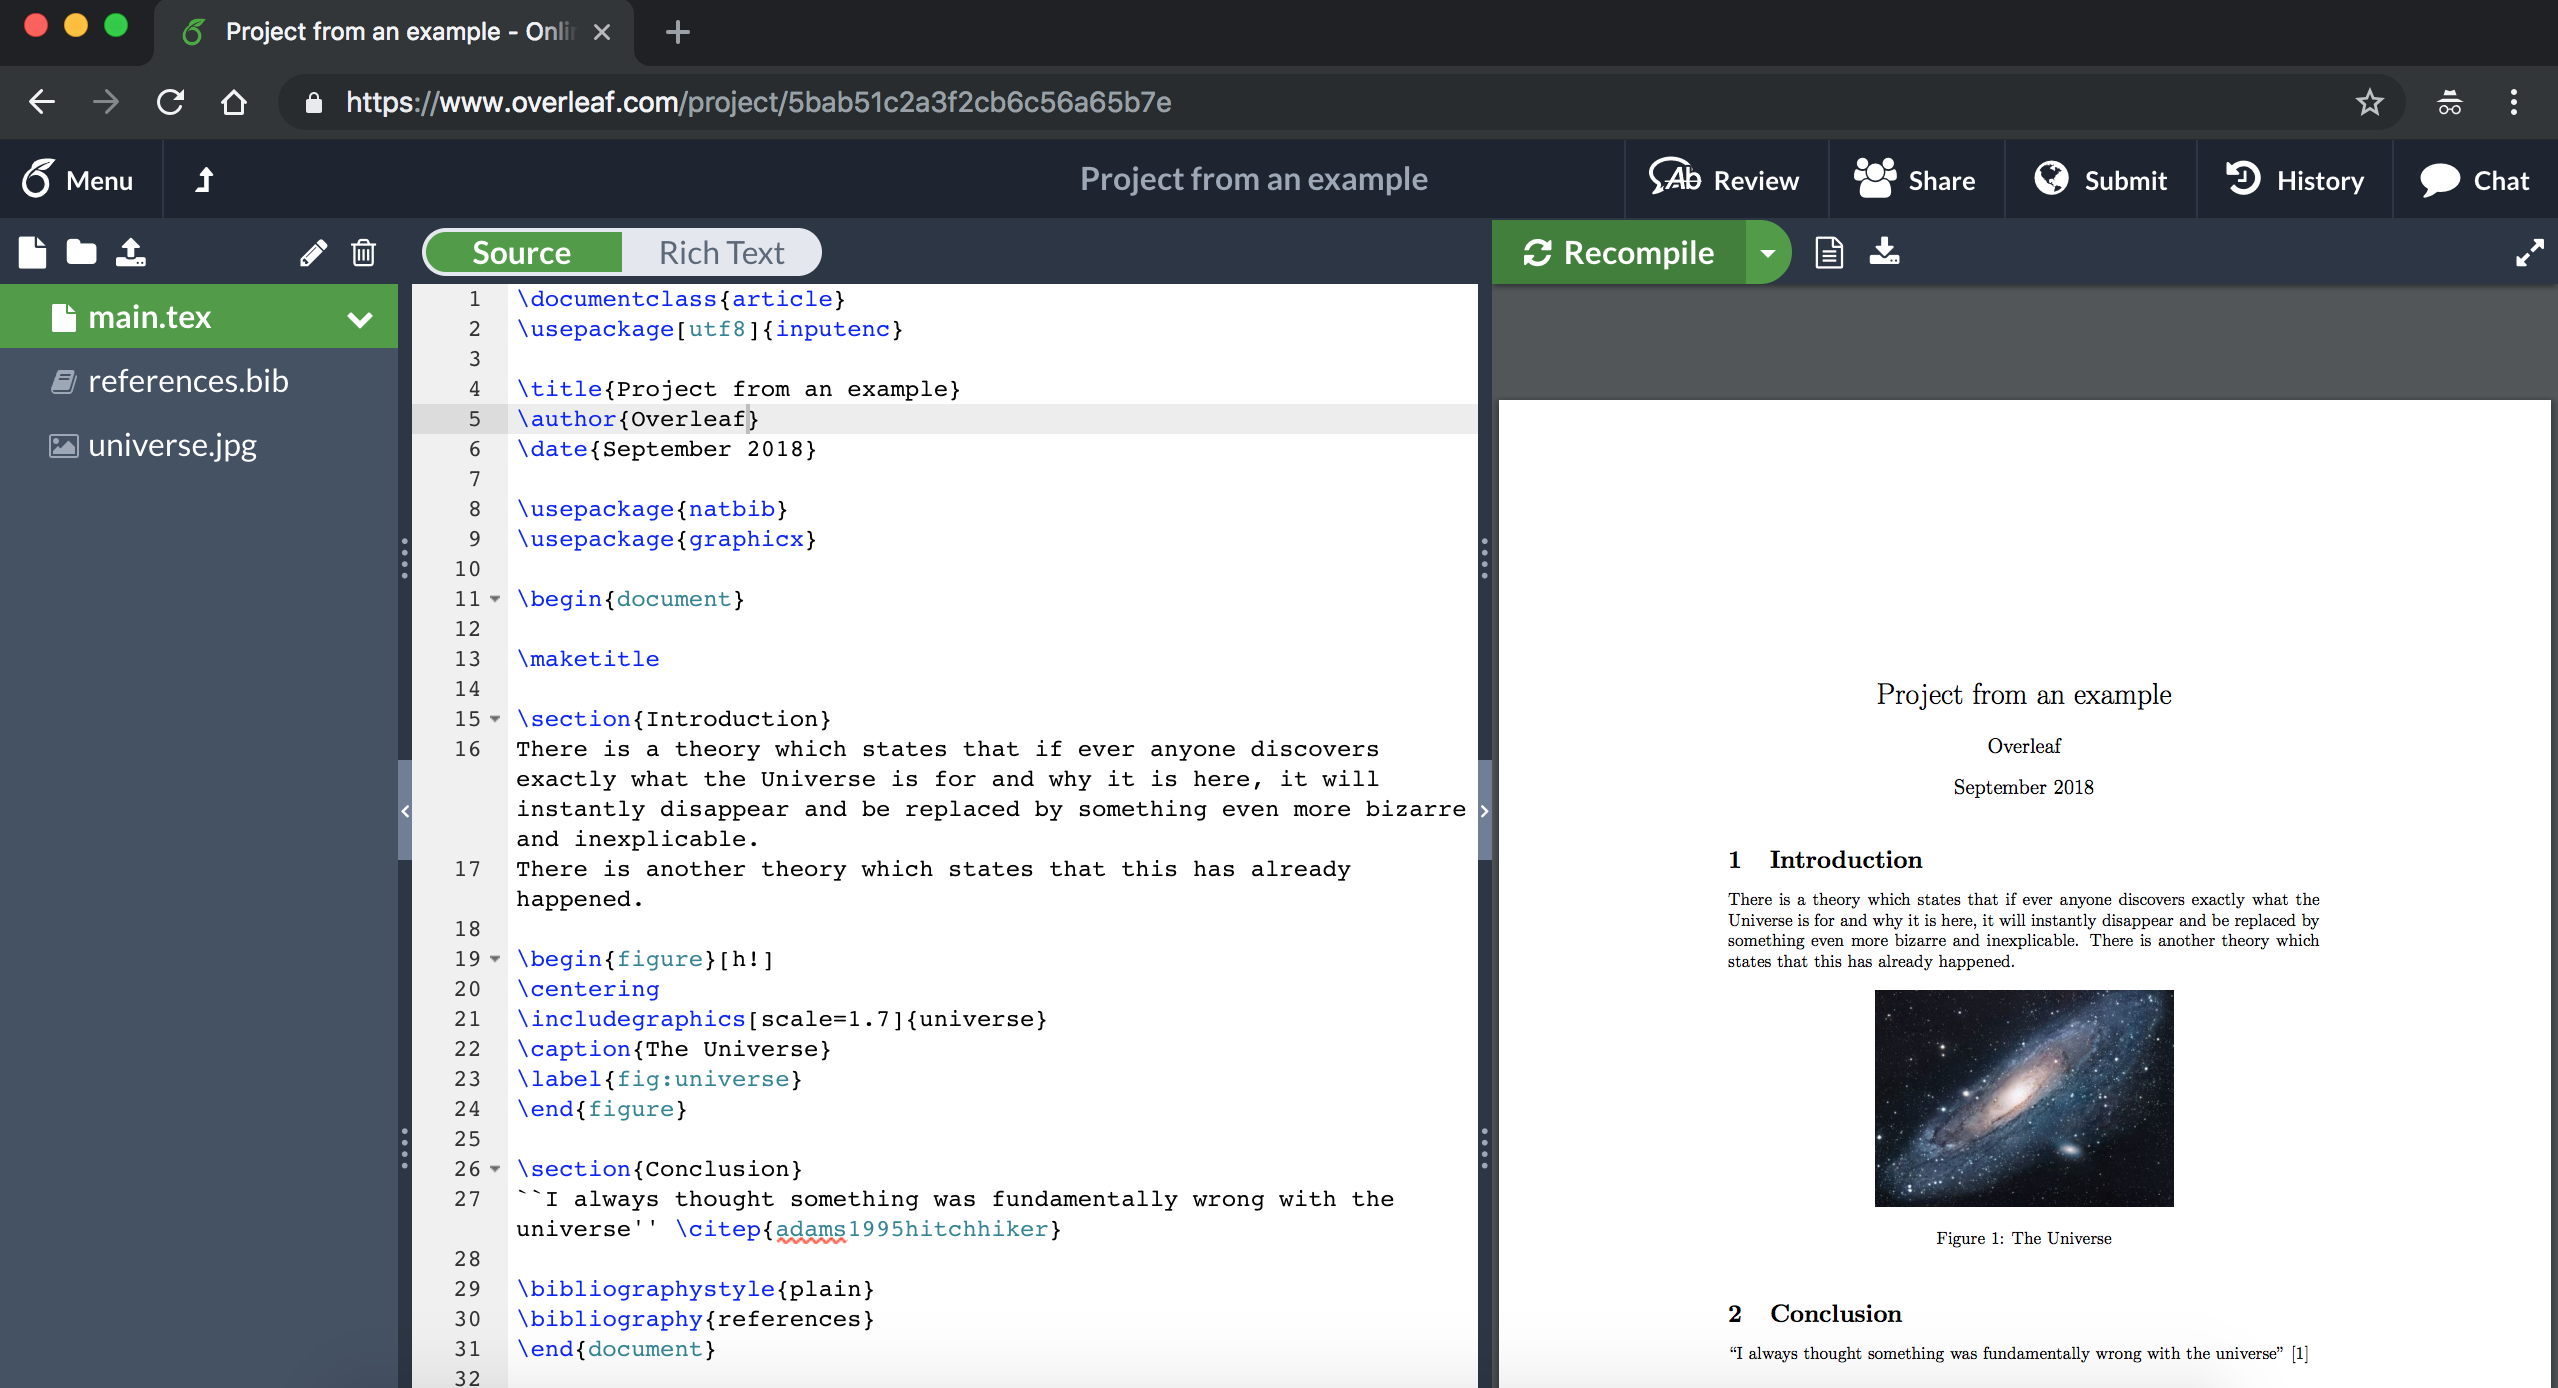
\includegraphics[width=0.99\textwidth]{figures/overleafEditor}
    \caption{The \LaTeX \ editor Overleaf, along with a preview of the document being authored, from~\cite{overleafDocs}}
    \label{fig:overleafPreview}
\end{figure}

    \chapter{Cryptography and Distributed Ledgers Background}\label{ch:crypto-background}

This chapter is dedicated to background on cryptography primitives and distributed ledgers.
While such concepts are not required to understand the semantics or the implementation of Confis, they are helpful to understand blockchain-based smart contracts (an application of the original concept by Szabo~\cite{szabo1997smart-contracts}) which are discussed in~\autoref{sec:ethereum} and are a significant part of the state of the art when it comes to machine-readable of agreements between parties -- which does concern this project.


\section{Cryptography Primitives}\label{sec:cryptography}

\subsection{Hash Functions}\label{subsec:crypto:hash}

Hash functions are cryptographic functions designed to behave like random
functions~\cite{smart2016randomOracleModel}.
When building a security proof, they can be assumed to have the following properties~\cite{smart2016randomOracleModel,
    smart2016hashFunctions}:
% FIXME needs references
\begin{description}
    \item[Determinism] A hash function always produces the same output for the same input
    \item[One-way] It is computationally impossible to compute the preimage for some output of a hash function
    \item[Uniformity] Outputs of a hash function are expected to be uniformly distributed.
    In practice, the output space of a hash function is finite, so \textit{collisions} (where two inputs produce the
    same output) are possible, but uniformity ensures this is an unlikely scenario.
\end{description}

\subsection{Public Key Cryptography}\label{subsec:crypto:pubkey}

In public key cryptography, two communicating parties (say Alice and Bob) can communicate privately by using pairs of
numbers that are related mathematically and which allow converting cleartext into cyphertext and
back~\cite{smart2016publicKey}.
This pair of numbers is called an asymmetric keypair, and is composed of a \textbf{public key} $e$ and a \textbf{private
key} $d$.

In this example, if Alice wishes to communicate with Bob, Bob can generate a keypair $(d, e)$ and publish $e$.
Alice can then encrypt her cleartext with $e$, and only Bob will be able to decrypt it (because only Bob knows $d$).


Conversely, the same keypair can be used by Bob to send a message to Alice where Alice can verify that only Bob
could have written the message.
This is called \textit{signing}~\cite{smart2016signatures} and, more generally, it allows a sender of a message to
prove they are the authors of the message to a recipient.

\subsection{Secure Digital Timestamps}\label{subsec:crypto:timestamps}
% TODO citation for definiton
\textit{Trusted (digital) timestamping} is the process of securely proving that a document (for our purposes, a blob of
bytes) was created, was modified at, or existed at a certain point in time.
% TODO citation for widely used
In industry this is commonly implemented by trusting a Time Stamping Authority (TSA)~\cite{timestamps_tsp_rfc} that
signs (see~\nameref{subsec:crypto:pubkey}) a concatenation of the hash of the document and a timestamp representing some
time $t$.
Therefore, a party that trusts the TSA to provide the right timestamp can verify that, when the TSA made the signature,
the current time was $t$.

This method can be used for confidential data because the TSA does not perform the hashing of the original document
themselves - they are exposed only to its digest.

Additionally, the requester of the timestamp cannot deny they were not in possession of the original data at the time
% TODO verify statement
$t$ given by the timestamp, because it was them that produced its hash digest.

\subsubsection{Decentralised Timestamps}

Secure timestamps can also be achieved without relying on trusted parties by publishing the document digest to a
blockchain~\cite{gipp2015timestamps_btc}: blocks are public and cannot be tampered with (see~\nameref{subsec:btc:pow}),
so putting a signed digest in a block shows that the signer knew the original document at the time the block was
accepted by the network.


\section{Bitcoin Protocol}\label{sec:bitcoin}

Blockchain technology was introduced in~\cite{nakamoto2008bitcoin} as a decentralised system allowing for electronic
cash payments.
Blockchains are immutable distributed ledgers where participants' balances can be verified by every other participant,
and it is computationally hard to tamper with balances to perform attacks (such as performing a transaction where a
participant spends more funds than what they own).

I will provide a brief overview of how Bitcoin provides these guarantees.

\subsection{Transactions}\label{subsec:btc:txs}

\cite{nakamoto2008bitcoin} defines an \textit{electronic coin} as a chain of signatures: a payer can use their private
key, the hash of the previous transaction, and the payee's public key to create a signed hash that can be verified by
the payee (and used by them for \textit{their} next transaction).
This is illustrated in Figure~\ref{fig:bitcoin-tx}.

\begin{figure}[th]
    \centering
    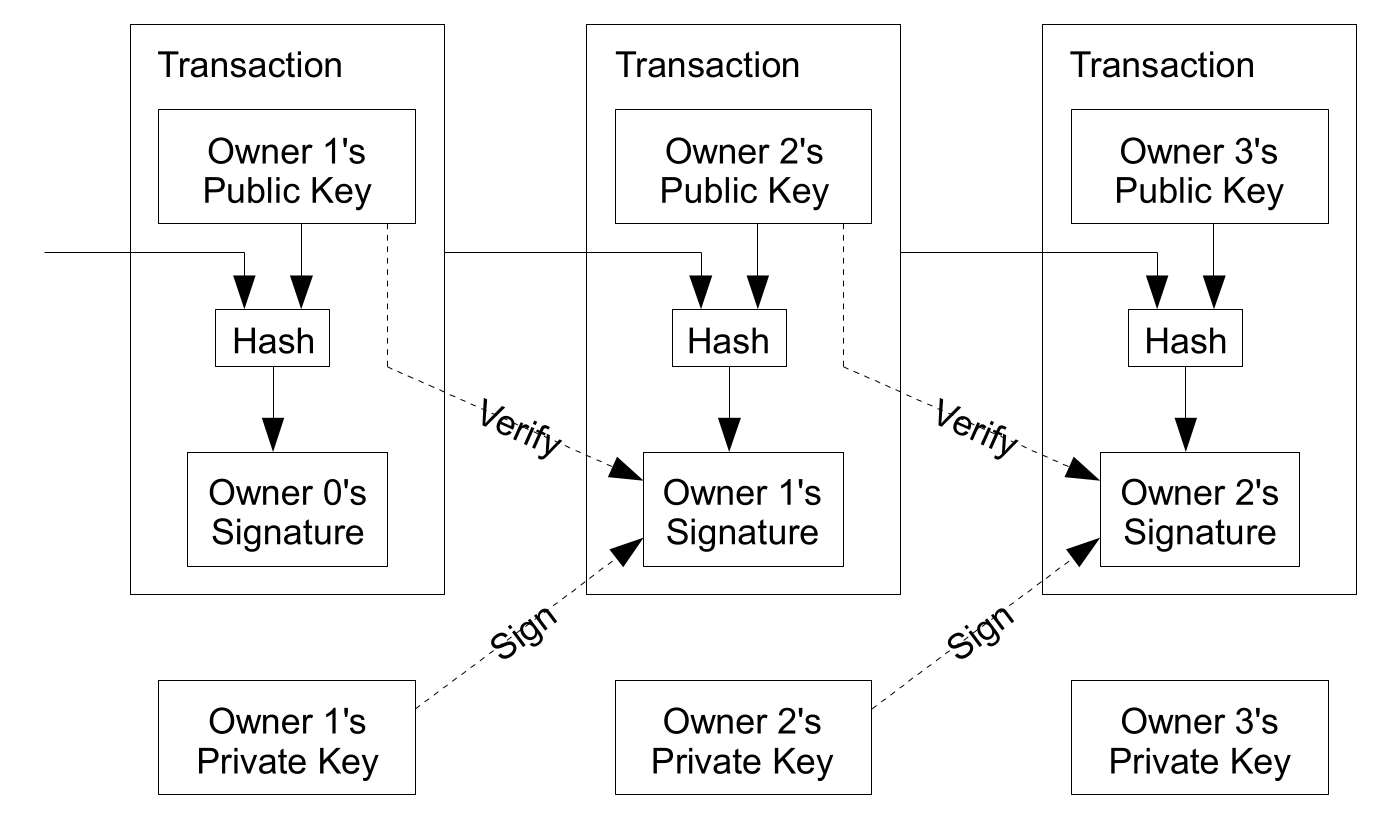
\includegraphics[width=0.8\columnwidth]{figures/bitcoin-tx}
    \caption[Bitcoin coin ownership transfer]{Transfer of ownership signature chain, from~\cite{nakamoto2008bitcoin}}
    \label{fig:bitcoin-tx}
\end{figure}

This ensures that, as long as a participants sign transactions at most once:
\begin{itemize}
    \item By verifying the chain of signatures, every participant can verify which participant owns which coin
    \item Only the owner of a coin can initiate a transaction with that coin
\end{itemize}

Bitcoin enforces that participants can only sign transactions once thanks to its proof-of-work
(see~\ref{subsec:btc:pow}) algorithm.

\subsection{Proof-Of-Work}\label{subsec:btc:pow}

Bitcoin ensures 'unique signatures' in transactions by grouping transactions in immutable, public \textit{blocks}.
Participants can then verify a payer has not signed a hash of a single transaction twice by looking at all existing
transactions.

Blocks are made immutable by including in them a value (called a \textit{nonce}) and the hash of the previous block.
% TODO verify it is the hash of the entire block that must yield the zeroes (implementation detail really)
The protocol then accepts only blocks where the $n$ first bits of its hash are zeroes. \\

Thus, in order to publish a block a participant must do work to find a nonce such that the block's hash meets this
condition - then other participants can verify its validity with a single hash operation.
This guarantees that a block cannot be changed (ie, a new copy published) without redoing the computational work.
Because blocks are chained (they include the hash of the previous block), in order to modify a transaction in the past
an adversary needs to redo the computational work for every block since that transaction (see Figure
\ref{fig:bitcoin-blockchain}).
% TODO implementation of mining rewards
Additionally, participants that successfully find a suitable nonce and propose new blocks (also referred to as
\textit{miners}) are allowed to add a specific transaction to the block where they own a newly created coin (also
referred to as \textit{mining reward}).

\begin{figure}[th]
    \centering
    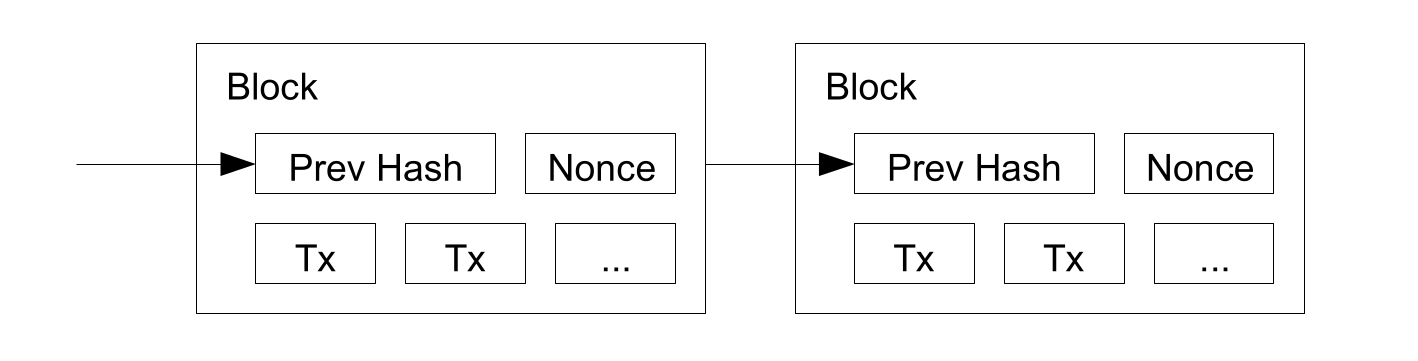
\includegraphics[width=0.8\columnwidth]{figures/bitcoin-blockchain}
    \caption[Two last blocks in a blockhain]{Two last blocks in a blockchain, from~\cite{nakamoto2008bitcoin}}
    \label{fig:bitcoin-blockchain}
\end{figure}

This model of consensus ensures that
\begin{itemize}
    \item Participants have a monetary incentive to stay honest with respect to the protocol
    \item An honest chain will out-compete an adversary's chain as long as the majority of computing power is honest
\end{itemize}

\subsection{Further details of the Bitcoin protocol}\label{subsec:btc.details}
\begin{figure}[th]
    \centering
    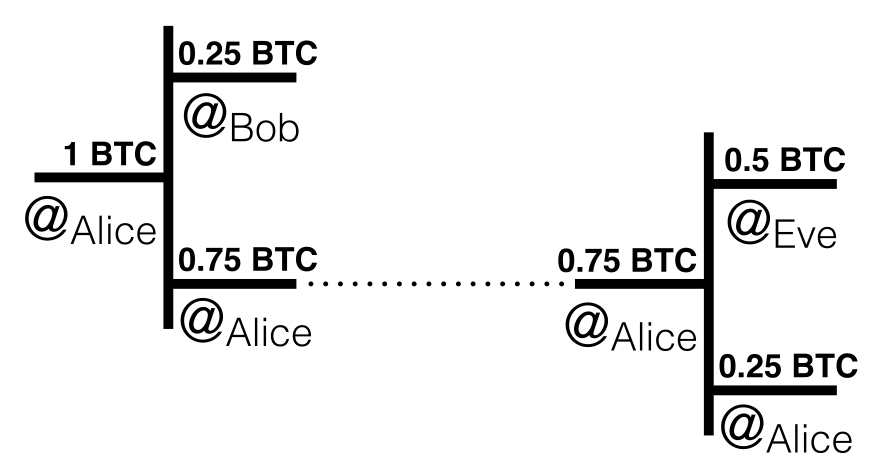
\includegraphics[width=0.6\columnwidth]{figures/bitcoin-2txs-outputs}
    \caption[Outputs and Inputs of two consecutive Transactions]{The outputs of a transaction correspond to
    the input of the next transaction (miner's fee not represented) from~\cite{gervais2022distribLedgers_transactionsInBitcoin}}
    \label{fig:bitcoin-2txs-outputs}
\end{figure}

While I provide a high-level overview of what makes the protocol function, there are many more details that combined
allow for more efficiency and usability:
\begin{itemize}
    \item Transactions may have several inputs and outputs, so participants can transfer amounts rather than single
    \textit{electronic coins}.
    When performing a payment, a typical transaction by Alice has two outputs: the amount she is paying Bob and the
    remainder, which makes up the rest of her funds (see Figure~\ref{fig:bitcoin-2txs-outputs}).
    Thus, a participant's balance is the sum of all the unspent outputs of previous transactions (the set of unspent
    outputs is commonly called the \textit{UTXO} set).
    \item By modifying how many of the leading bits of a blocks' hash must be zeroes, the average computation necessary
    to produce a new block can be adjusted by the protocol.
    \item By using Merkle Trees~\cite{merkle1980tree} transactions with fully spent transaction outputs can be discarded
    without breaking the block's hash.
    This allows compacting old blocks to reclaim disk space.
    \item A participant that does not wish to mine or hold a copy of the entire blockchain can still verify payments.
    It can keep a copy of the block headers of the longest chain and link a transaction to where it is on-chain and
    check that other network nodes have accepted it.
    This process is called \textit{Simple Payment Verification} (SPV)~\cite{nakamoto2008bitcoin}.
    \item Miners have an additional incentive (other than the mining reward) to verify transactions: the
    \textit{transaction fee}.
    The difference of the sum of a transaction's inputs and the sum its outputs corresponds to the transaction fee, which
    goes to the miner.
    \[
        \text{fee}_\text{miner} = \sum{\text{inputs}} - \sum{\text{outputs}}
    \]
    This provides an incentive for the miner to place this specific transaction in the block they propose.
\end{itemize}

For more information on all the workings of the Bitcoin protocol, please refer to~\cite{nakamoto2008bitcoin}.


    \printbibliography[heading=bibintoc]

\end{document}

